% Verifying the Verse -- IEEE conference paper.
% Build: latexmk -lualatex main.tex   (LuaLaTeX is needed for the Arabic text; see README.md in this folder)
\documentclass[conference]{IEEEtran}

% ---------------------------------------------------------------- fonts and languages
\usepackage{fontspec}
\setmainfont{TeX Gyre Termes}
\usepackage[english,bidi=basic]{babel}
\babelprovide[import]{arabic}
\babelfont[arabic]{rm}[Renderer=HarfBuzz,Scale=1.05]{Amiri}

% ---------------------------------------------------------------- packages
\usepackage{amsmath,amssymb}
\usepackage{booktabs}
\usepackage{multirow}
\usepackage{array}
\usepackage{tabularx}
\usepackage{graphicx}
\usepackage{xcolor}
\usepackage{tikz}
\usetikzlibrary{arrows.meta,positioning,shapes.geometric,fit,calc,backgrounds}
\usepackage{algorithm}
\usepackage{algpseudocode}
\usepackage{cite}
\usepackage{url}
\usepackage[hidelinks]{hyperref}

% ---------------------------------------------------------------- macros
\newcommand{\ar}[1]{\foreignlanguage{arabic}{#1}}
% a result that is not available yet: shown in red so it cannot be missed
\newcommand{\pending}[1]{\textcolor{red}{\textbf{[#1]}}}
\newcommand{\TBD}{\pending{TBD}}
% numbers produced by scripts/analysis.py; a number that has not been produced yet prints as a red placeholder
\IfFileExists{generated/numbers.tex}{% generated by prosody-verifier/paper/scripts/analysis.py -- do not edit by hand
\newcommand{\gEoneStrictGivenBase}{10.51}
\newcommand{\gEzeroStrictGivenBase}{12.22}
\newcommand{\gRefStrictGivenBase}{57.89}
\newcommand{\kEoneBYesVNo}{39.33}
\newcommand{\kEoneVB}{0.241}
\newcommand{\kEzeroBYesVNo}{42.16}
\newcommand{\kEzeroLB}{0.657}
\newcommand{\kEzeroVB}{0.082}
\newcommand{\kRefBYesVNo}{15.57}
\newcommand{\kRefLB}{0.782}
\newcommand{\kRefVB}{0.186}
\newcommand{\lrBaseAIC}{8,724}
\newcommand{\lrBaseN}{10,443}
\newcommand{\lrBaseRsq}{0.307}
\newcommand{\lrExtAIC}{7,392}
\newcommand{\lrExtN}{10,443}
\newcommand{\lrExtRsq}{0.346}
\newcommand{\mCmrBaytOk}{81.64}
\newcommand{\mCmrBaytOkCI}{[80.5, 82.8]}
\newcommand{\mCmrCountExact}{100.00}
\newcommand{\mCmrCountExactCI}{[100.0, 100.0]}
\newcommand{\mCmrLenB}{0.00}
\newcommand{\mCmrLenC}{0.00}
\newcommand{\mCmrLenD}{0.00}
\newcommand{\mCmrMeterOk}{38.80}
\newcommand{\mCmrMeterOkCI}{[36.4, 41.3]}
\newcommand{\mCmrNoMarginStrict}{0.13}
\newcommand{\mCmrNoReading}{5.43}
\newcommand{\mCmrNoReadingCI}{[4.9, 6.0]}
\newcommand{\mCmrRhymeOk}{0.27}
\newcommand{\mCmrRhymeOkCI}{[0.1, 0.5]}
\newcommand{\mCmrStrictValid}{0.00}
\newcommand{\mCmrStrictValidCI}{[0.0, 0.0]}
\newcommand{\mCmrVsRefStrict}{-43.4 [-45.9, -40.9]}
\newcommand{\mCwmBaytOk}{0.57}
\newcommand{\mCwmBaytOkCI}{[0.4, 0.8]}
\newcommand{\mCwmCountExact}{100.00}
\newcommand{\mCwmCountExactCI}{[100.0, 100.0]}
\newcommand{\mCwmLenA}{0.00}
\newcommand{\mCwmLenB}{0.00}
\newcommand{\mCwmLenC}{0.00}
\newcommand{\mCwmLenD}{0.00}
\newcommand{\mCwmMeterOk}{0.00}
\newcommand{\mCwmMeterOkCI}{[0.0, 0.0]}
\newcommand{\mCwmNoMarginStrict}{1.69}
\newcommand{\mCwmNoReading}{83.57}
\newcommand{\mCwmNoReadingCI}{[82.5, 84.6]}
\newcommand{\mCwmRhymeOk}{93.13}
\newcommand{\mCwmRhymeOkCI}{[92.3, 93.9]}
\newcommand{\mCwmStrictValid}{0.00}
\newcommand{\mCwmStrictValidCI}{[0.0, 0.0]}
\newcommand{\mCwmVsRefStrict}{-54.9 [-56.5, -53.3]}
\newcommand{\mEoneBaytOk}{44.20}
\newcommand{\mEoneBaytOkCI}{[43.0, 45.4]}
\newcommand{\mEoneBilstmBaytOk}{82.07}
\newcommand{\mEoneBilstmBaytOkCI}{[81.1, 83.0]}
\newcommand{\mEoneCountExact}{82.07}
\newcommand{\mEoneCountExactCI}{[80.8, 83.4]}
\newcommand{\mEoneLenA}{10.13}
\newcommand{\mEoneLenB}{1.24}
\newcommand{\mEoneLenC}{0.21}
\newcommand{\mEoneLenD}{0.00}
\newcommand{\mEoneMeterOk}{8.91}
\newcommand{\mEoneMeterOkCI}{[7.9, 9.8]}
\newcommand{\mEoneNoMarginStrict}{8.91}
\newcommand{\mEoneNoReading}{32.01}
\newcommand{\mEoneNoReadingCI}{[31.0, 33.0]}
\newcommand{\mEoneRhymeOk}{36.31}
\newcommand{\mEoneRhymeOkCI}{[34.8, 37.9]}
\newcommand{\mEoneStrictValid}{5.17}
\newcommand{\mEoneStrictValidCI}{[4.4, 5.9]}
\newcommand{\mEoneVsRefBilstm}{-15.2 [-16.3, -14.2]}
\newcommand{\mEoneVsRefStrict}{-49.8 [-51.4, -48.1]}
\newcommand{\mEzeroBaytOk}{53.78}
\newcommand{\mEzeroBaytOkCI}{[52.6, 54.9]}
\newcommand{\mEzeroBilstmBaytOk}{95.37}
\newcommand{\mEzeroBilstmBaytOkCI}{[95.0, 95.8]}
\newcommand{\mEzeroBindBayt}{40.41}
\newcommand{\mEzeroBindStrict}{5.06}
\newcommand{\mEzeroCountExact}{83.40}
\newcommand{\mEzeroCountExactCI}{[82.2, 84.6]}
\newcommand{\mEzeroLenA}{17.51}
\newcommand{\mEzeroLenB}{2.24}
\newcommand{\mEzeroLenC}{0.63}
\newcommand{\mEzeroLenD}{0.00}
\newcommand{\mEzeroMeterOk}{15.51}
\newcommand{\mEzeroMeterOkCI}{[14.3, 16.7]}
\newcommand{\mEzeroNoMarginStrict}{13.56}
\newcommand{\mEzeroNoReading}{25.82}
\newcommand{\mEzeroNoReadingCI}{[25.0, 26.7]}
\newcommand{\mEzeroRhymeOk}{38.18}
\newcommand{\mEzeroRhymeOkCI}{[36.6, 39.8]}
\newcommand{\mEzeroStrictValid}{8.99}
\newcommand{\mEzeroStrictValidCI}{[8.0, 9.9]}
\newcommand{\mEzeroVsRefBilstm}{-1.9 [-2.6, -1.2]}
\newcommand{\mEzeroVsRefStrict}{-45.9 [-47.7, -44.2]}
\newcommand{\mRefBaytOk}{82.09}
\newcommand{\mRefBaytOkCI}{[81.0, 83.2]}
\newcommand{\mRefBilstmBaytOk}{97.30}
\newcommand{\mRefBilstmBaytOkCI}{[96.7, 97.8]}
\newcommand{\mRefBindBayt}{80.85}
\newcommand{\mRefBindStrict}{52.48}
\newcommand{\mRefCountExact}{100.00}
\newcommand{\mRefCountExactCI}{[100.0, 100.0]}
\newcommand{\mRefLenA}{70.50}
\newcommand{\mRefLenB}{50.19}
\newcommand{\mRefLenC}{41.44}
\newcommand{\mRefLenD}{25.42}
\newcommand{\mRefMeterOk}{57.08}
\newcommand{\mRefMeterOkCI}{[55.5, 58.7]}
\newcommand{\mRefNoMarginStrict}{69.72}
\newcommand{\mRefNoReading}{5.18}
\newcommand{\mRefNoReadingCI}{[4.6, 5.7]}
\newcommand{\mRefRhymeOk}{93.13}
\newcommand{\mRefRhymeOkCI}{[92.3, 93.9]}
\newcommand{\mRefStrictValid}{54.93}
\newcommand{\mRefStrictValidCI}{[53.3, 56.5]}
\newcommand{\mcEoneChi}{1,646.4}
\newcommand{\mcEoneP}{$<$0.001}
\newcommand{\mcEzeroChi}{1,473.7}
\newcommand{\mcEzeroP}{$<$0.001}
\newcommand{\nestBaseSOneRsq}{0.174}
\newcommand{\nestBaseSThreeRsq}{0.307}
\newcommand{\nestBaseSTwoRsq}{0.300}
\newcommand{\nestExtSOneRsq}{0.262}
\newcommand{\nestExtSThreeRsq}{0.346}
\newcommand{\nestExtSTwoRsq}{0.337}
\newcommand{\ourBestLoss}{2.3205}
\newcommand{\ourBestStep}{2400}
\newcommand{\ourInitLoss}{3.0589}
\newcommand{\ourSteps}{4,236}
\newcommand{\ourTestLoss}{2.3147}
\newcommand{\paperBestLoss}{2.2074}
\newcommand{\paperShaerBaseMeterAccuracyPct}{95.17}
\newcommand{\paperShaerCountAdherence}{0.9792}
\newcommand{\paperShaerExactCountAccuracyPct}{83.40}
\newcommand{\paperShaerMeterConformity}{0.9064}
\newcommand{\paperTestLoss}{2.1932}
\newcommand{\paperYehiaBaseMeterAccuracyPct}{26.49}
\newcommand{\paperYehiaCountAdherence}{0.7680}
\newcommand{\paperYehiaExactCountAccuracyPct}{44.47}
\newcommand{\paperYehiaMeterConformity}{0.1494}
\newcommand{\powDev}{0.995}
\newcommand{\powMDE}{1.7}
\newcommand{\powNFive}{312}
\newcommand{\powNFiveWide}{626}
\newcommand{\powNTen}{155}
\newcommand{\repEOneAcc}{80.15}
\newcommand{\repEOneAdh}{0.9764}
\newcommand{\repEOneConf}{0.6613}
\newcommand{\repEOneExact}{82.07}
\newcommand{\repEThreeAcc}{78.63}
\newcommand{\repEThreeAdh}{0.9833}
\newcommand{\repEThreeConf}{0.6324}
\newcommand{\repEThreeExact}{85.29}
\newcommand{\repETwoAcc}{26.86}
\newcommand{\repETwoAdh}{0.7549}
\newcommand{\repETwoConf}{0.1435}
\newcommand{\repETwoExact}{42.32}
\newcommand{\repEZeroAcc}{95.17}
\newcommand{\repEZeroAdh}{0.9792}
\newcommand{\repEZeroConf}{0.9064}
\newcommand{\repEZeroExact}{83.40}
\newcommand{\vCmrAnyForm}{0.00}
\newcommand{\vCmrBaseBilstm}{0.00}
\newcommand{\vCmrFull}{0.00}
\newcommand{\vCmrMarginOne}{0.00}
\newcommand{\vCmrMarginThree}{0.13}
\newcommand{\vCmrNoLength}{0.00}
\newcommand{\vCmrNoMargin}{0.13}
\newcommand{\vCmrNoRhyme}{38.80}
\newcommand{\vCwmAnyForm}{0.03}
\newcommand{\vCwmBaseBilstm}{0.00}
\newcommand{\vCwmFull}{0.00}
\newcommand{\vCwmMarginOne}{0.00}
\newcommand{\vCwmMarginThree}{0.49}
\newcommand{\vCwmNoLength}{0.00}
\newcommand{\vCwmNoMargin}{1.69}
\newcommand{\vCwmNoRhyme}{0.00}
\newcommand{\vEoneAnyForm}{5.23}
\newcommand{\vEoneBaseBilstm}{45.94}
\newcommand{\vEoneFull}{5.17}
\newcommand{\vEoneMarginOne}{4.91}
\newcommand{\vEoneMarginThree}{6.89}
\newcommand{\vEoneNoLength}{5.17}
\newcommand{\vEoneNoMargin}{8.91}
\newcommand{\vEoneNoRhyme}{8.62}
\newcommand{\vEzeroAnyForm}{9.16}
\newcommand{\vEzeroBaseBilstm}{73.14}
\newcommand{\vEzeroBinding}{5.06}
\newcommand{\vEzeroFull}{8.99}
\newcommand{\vEzeroMarginOne}{8.36}
\newcommand{\vEzeroMarginThree}{11.92}
\newcommand{\vEzeroNoLength}{9.11}
\newcommand{\vEzeroNoMargin}{13.56}
\newcommand{\vEzeroNoRhyme}{14.97}
\newcommand{\vRefAnyForm}{57.20}
\newcommand{\vRefBaseBilstm}{94.34}
\newcommand{\vRefBinding}{52.48}
\newcommand{\vRefFull}{54.93}
\newcommand{\vRefMarginOne}{50.96}
\newcommand{\vRefMarginThree}{66.04}
\newcommand{\vRefNoLength}{54.93}
\newcommand{\vRefNoMargin}{69.72}
\newcommand{\vRefNoRhyme}{57.08}
\newcommand{\lrSystems}{E0, E1}
}{}
\newcommand{\val}[1]{\ifcsname #1\endcsname\csname #1\endcsname\else\TBD\fi}
\newcommand{\pp}{\,pp}
% table rows written by scripts/analysis.py (the TeX primitive \input works inside tabular)
\makeatletter\newcommand{\rowsinput}[1]{\@@input #1 }\makeatother
\newcommand{\Hyp}[1]{\textbf{H#1}}
\graphicspath{{generated/}{figures/}}

\begin{document}

\title{Verifying the Verse: Reproducing Shaer and Extending Controlled Arabic Poetry Generation with a Formal Prosody Verifier}

\author{\IEEEauthorblockN{Muhammad Shahbaz}
\IEEEauthorblockA{\pending{Department, University}\\
\pending{City, Country}\\
\pending{email}}}

\maketitle

\begin{abstract}
Large language models can now be asked for a classical Arabic poem in a given meter and length, and Shaer, a recent
fine-tuned model, reports that 95.17\% of its poems are in the requested meter. That figure comes from a neural meter
classifier that looks at each verse separately. We asked two questions: can the result be reproduced, and does it mean
that the poems are metrically correct? We re-ran the whole Shaer pipeline on Google Colab GPUs. Re-scoring the released
poems reproduced every published number exactly, but poems that we generated again with the released adapter reached
\val{repEOneAcc}\% base-meter accuracy, and our re-trained model \val{repEThreeAcc}\%. We then built a rule-based verifier of
classical prosody (\emph{\textquotesingle ar\=u\d{d}}) that scans every hemistich against the derived patterns of 16 meters
and also checks rhyme and length. Under this strict criterion only \val{mEzeroStrictValid}\% of the released poems are
fully valid, against \val{mRefStrictValid}\% of the human poems written for the same prompts, and validity falls sharply
with poem length. Among the verses the classifier accepts, \val{mEzeroNoReading}\% of Shaer's have a hemistich with no
reading at all in the requested meter. A logistic model, nested-model comparisons and controls confirm the pattern. We
then describe and pre-register three extensions that use the verifier during generation and training (hemistich search,
self-training and a quality study); their results are reported as placeholders until the runs finish. The study shows
that a lenient metric can hide most formal errors and offers a reusable, open verifier for Arabic verse.
\end{abstract}

\begin{IEEEkeywords}
Arabic poetry generation, prosody, \textquotesingle ar\=u\d{d}, meter verification, controlled text generation,
reproducibility, large language models, evaluation
\end{IEEEkeywords}

\section{Introduction}
\label{sec:intro}

Classical Arabic poetry is written in lines called \emph{bayts}. Each bayt has two halves, or hemistichs, and every
hemistich must follow one of sixteen quantitative meters, the \emph{bu\d{h}\=ur}, codified in the eighth century by
al-Khal\={\i}l ibn A\d{h}mad~\cite{frolov2000classical}. Every bayt of a poem must also end on the same rhyme letter,
the \emph{raw\={\i}}. These rules are strict. A reader trained in the tradition hears a missing syllable at once, and
a teacher of Arabic literature will reject a poem with one broken hemistich. A system that claims to write classical
Arabic verse therefore has a clear and checkable target.

Large language models (LLMs) have made such systems easy to build. Shaer~\cite{abbas2026shaer} fine-tunes the Arabic
model Yehia-7B~\cite{yehia2025} with QLoRA~\cite{dettmers2023qlora} on 116,032 poems from the Ashaar
corpus~\cite{alyafeai2023ashaar}. A prompt names the meter, its sub-form, the number of hemistichs and a topic
description, and the model writes the poem. The authors report a base-meter accuracy of 95.17\% and an exact length
accuracy of 83.40\% on 3,481 held-out prompts, far above general Arabic models such as Fanar~\cite{fanar2026fanar2}.

The meter numbers come from a bidirectional LSTM (BiLSTM) classifier~\cite{abandah2022classifying} that reads one
bayt at a time and outputs the most likely meter. A classifier of this kind is trained to tell the sixteen meters
apart. It is not trained to say ``this is not a meter at all''. A bayt that is one syllable short of al-K\=amil is
still closer to al-K\=amil than to any other meter, so the classifier will label it al-K\=amil with high confidence.
High accuracy under this metric may therefore hide many unmetrical lines. Rhyme is not checked at all.

This paper is an empirical study of that gap. We first \emph{reproduce} Shaer end to end on Google Colab GPUs, and
then \emph{extend} its evaluation with a formal verifier of Arabic prosody, which we use to measure how often the
poems are actually correct and to guide generation and training. We ask three research questions:
\begin{itemize}
\item \textbf{RQ1 (reproduction).} Can Shaer's published results be reproduced from its released code, data and
adapter, and where do the numbers differ?
\item \textbf{RQ2 (measurement).} How often are the generated poems strictly valid in meter, rhyme and length, and how
far does the classifier-based metric overstate this?
\item \textbf{RQ3 (improvement).} Can the verifier raise strict validity when it is used at decoding time or to select
training data, without hurting the quality of the poems?
\end{itemize}

\textbf{Contributions.} The paper makes the following contributions.
\begin{enumerate}
\item \emph{An independent reproduction} of Shaer (released poems, released adapter, untuned base model and a full
re-training), reported next to the published numbers with an explanation of every difference
(Section~\ref{sec:res-repro}).
\item \emph{A formal, open verifier of classical Arabic prosody} that derives 1,867 hemistich patterns of 16 meters
from the classical rules, scans undiacritised or partly diacritised text with a pronunciation prior, and checks
rhyme (raw\={\i}, its vowel, \emph{ridf}, \emph{ta'\={\i}s}) and length (Section~\ref{sec:m1}).
\item \emph{A strict re-scoring} of the reproduced systems and of the human poems, showing that strict validity is far
below what the classifier metric suggests and that it falls with poem length (Section~\ref{sec:results}).
\item \emph{A robustness analysis} with nested logistic models, nested definitions of validity, alternative settings
and control samples (Section~\ref{sec:robust}).
\item \emph{Three pre-registered extensions}: verifier-guided hemistich search compared with best-of-$N$ sampling at
equal compute, self-training on verifier-approved poems, and a quality study with an LLM judge and blinded human
raters. Their designs and predictions were fixed before the runs (Sections~\ref{sec:m4}--\ref{sec:m6}).
\end{enumerate}

The rest of the paper is organised as follows. Section~\ref{sec:lit} reviews related work and states the hypotheses.
Section~\ref{sec:background} introduces the prosody needed to read the paper. Section~\ref{sec:methods} describes the
techniques M0--M6 with examples from the data. Sections~\ref{sec:design} and~\ref{sec:setup} give the research
design and the analysis setup. Sections~\ref{sec:results} and~\ref{sec:robust} report the results and the robustness
checks. Section~\ref{sec:case} discusses a practical case, Section~\ref{sec:ethics} ethics and limitations, and
Section~\ref{sec:conclusion} concludes.

\section{Literature Review and Hypotheses}
\label{sec:lit}

\subsection{How the literature was collected}
The review draws on a systematic literature search that we carried out for a wider project on poetry generation in
Arabic-script languages, following the PRISMA~2020 flow. Search strings for generation, meter, rhyme, evaluation and
low-resource languages were run on Semantic Scholar, arXiv, the ACL Anthology and Crossref. They returned 33,279
records, of which 19,213 were unique. Automated rules (a Boolean match and a computational-study filter) kept 5,531 for
title and abstract screening, and forward and backward snowballing from 21 seed papers added further candidates. In
total 1,040 studies from 2024 to 2026 were included and graded by closeness to the topic: 55 core, 228 high and 757
related. For this paper we read the core and high studies on our six aspects and kept the 40 closest. We added a few
earlier foundational works (Deep-speare, PoeLM, ByGPT5) and the methods we borrow from other fields (verifiers,
self-training, statistics). The 40 studies are grouped into six themes below. Where we read only an abstract, we
report only what the abstract states.

\subsection{Theme A: Form-controlled poetry generation}
Early neural systems learned meter and rhyme jointly with the language model. Deep-speare~\cite{lau2018deepspeare}
trained separate meter and rhyme components for English sonnets, and PoeLM~\cite{ormazabal2022poelm} put control codes
for syllable counts and rhyme into the prompt of a Spanish and Basque language model, filtering samples afterwards.
ByGPT5~\cite{belouadi2023bygpt5} showed that a token-free (byte-level) model controls meter and rhyme better than a
subword model of similar size, and CharPoet~\cite{yu2024charpoet} and GPT Czech Poet~\cite{chudoba2024gptczechpoet}
reached the same conclusion for Chinese and Czech: when the unit of the form is a character or a syllable, a tokeniser
that splits words into arbitrary pieces makes control harder. Liao and Shi~\cite{liao2026tokenization} give a
direct measurement of this effect, showing that subword tokenisation weakens a model's knowledge of rhyme and
syllables.

Other work places the form outside the language model. PoetryDiffusion~\cite{hu2024poetrydiffusion} uses a separately
trained metrical controller to steer a diffusion model at every denoising step, with a per-position template for line
ends. PoeTone~\cite{qu2025poetone} evaluates 18 LLMs on Chinese \emph{Songci} templates and adds a Generate--Critic loop
that keeps the best of several candidates. BIPro~\cite{zou2025bipro} constrains generation block by block through
inverse prompting, and Chakrabarty et al.~\cite{chakrabarty2022helpme} show that instruction tuning lets a model
follow form requests written in plain language. Across these studies the form is either learned or checked by a
component that is itself learned; a deterministic rule-based checker inside the loop is rare.

\subsection{Theme B: Arabic and quantitative-meter generation}
Shaer~\cite{abbas2026shaer}, our base paper, is the closest work. It conditions Yehia-7B on a meter sub-form, a
hemistich count and a topic description, trains with QLoRA and completion-only loss, and evaluates meter with the
BiLSTM of Abandah et al.~\cite{abandah2022classifying}. The authors also release adapters trained with reinforcement
learning against that classifier. Fanar-Diwan, part of the Fanar~2.0 stack~\cite{fanar2026fanar2}, conditions classical
poetry on meter, rhyme, topic, era and poet. Ashaar~\cite{alyafeai2023ashaar} provides the corpus and an earlier
generator. Sadallah et al.~\cite{sadallah2026instructpoet} build instruction data for writing, revising and continuing
poems in Arabic and its dialects under style and rhyme criteria. Ta\d{h}dh\={\i}b~\cite{elzohbi2025tahdib} is the
only Arabic work we found that uses a rule-based rhythm: it maps diacritised script to beats with rules and fills
phrases with a byte-level model to hit a target rhythm.

Sanskrit, whose meters are also quantitative, gives the strongest evidence for checking at decoding time.
Chandomitra~\cite{jagadeeshan2026chandomitra} reports that constrained decoding raises metrical validity to 99.86\%
while GPT-4o with one example reaches 31\%, and Pingala~\cite{jagadeeshan2026pingala} decodes over syllable-weight
patterns and gains further by working in a phonetic transliteration. Low-resource Perso-Arabic and South Asian work
follows the same direction with smaller models: UPON~\cite{tabassam2025upon} generates Urdu couplets in one meter and
filters them with a rule-based scansion tool, Pashto generation~\cite{ullah2024pashto} fine-tunes small transformers,
and Bangla form-aware generation~\cite{amina2025bangla} uses control tokens for meter, rhyme and line boundaries.

\subsection{Theme C: Computational prosody and meter classification}
Most Arabic work on meter is classification. Abandah et al.~\cite{abandah2022classifying} classify and diacritise
poems with recurrent networks, Mutawa and Alrumaih~\cite{mutawa2025arabicmeter} compare deep character-level
classifiers over the 16 meters, and AraPoemBERT~\cite{qarah2024arapoembert} pre-trains a model on poetry and fine-tunes
it for meter and sub-form. These systems choose the most likely meter among a closed set. They do not decide whether a
line is metrical, and they do not say where it breaks. Rule-based scansion exists for neighbouring traditions:
UPMVM~\cite{zaman2025upmvm} verifies Urdu meters with finite automata over 290 meters and sub-meters, Persian prosody
recognition~\cite{shahrestani2025persianprosody} and the Chaame rhyme and \emph{radif}
dataset~\cite{rezaei2026chaame} address Persian, and De Sisto et al.~\cite{desisto2024poetrytools} survey open
scansion and rhyme tools across languages. The systematic review of Alharthi~\cite{alharthi2026arabicpoetryslr} lists
the tasks, data sets and evaluation practice of Arabic poetry NLP. The rules themselves are documented in classical
and modern prosody textbooks such as Frolov~\cite{frolov2000classical}.

\subsection{Theme D: Constraints, verifiers and test-time compute}
Controlled text generation has two broad families. Decoding-time methods change the next-token distribution or the
search: FUDGE~\cite{yang2021fudge} reweights tokens with a discriminator of the future, and NeuroLogic
decoding~\cite{lu2021neurologic} keeps beams that satisfy lexical constraints. Sampling settings such as nucleus
sampling~\cite{holtzman2020curious} decide how diverse each candidate is. In reasoning tasks, a separate
\emph{verifier} that scores whole solutions~\cite{cobbe2021verifiers} or each step~\cite{lightman2024verify} raises
accuracy when the model is sampled several times, and Snell et al.~\cite{snell2025scaling} show that how the extra
test-time compute is spent (parallel samples or guided search) matters as much as its amount. Poetry has the rare
property that a step-level verifier can be exact: a hemistich either scans or it does not. This is the idea behind our
hemistich search (Section~\ref{sec:m4}), and it is why we compare it with best-of-$N$ at the same compute.

\subsection{Theme E: Refinement, reinforcement learning and self-training}
A checker can also improve the model itself. STaR~\cite{zelikman2022star}, rejection-sampling fine-tuning~\cite{yuan2023rft}
and ReST~\cite{gulcehre2023rest} fine-tune a model on its own outputs that pass a check, and GRPO~\cite{shao2024deepseekmath}
uses group-relative rewards. In poetry, Xunzi Yayun R1~\cite{zhao2025xunziyayun} trains with GRPO and rule-based rewards
for tone, rhyme, parallelism and length, and Progressive Structural Internalization~\cite{li2026psi} first scaffolds the
format and then removes the scaffold with cascaded reinforcement learning. Refinement loops fix a poem after it is
written: Agirrezabal and Gon\c{c}alo Oliveira~\cite{agirrezabal2025refining} feed the output of an LLM or rule-based
metrical evaluator back to the generator and find that feedback helps in both cases, and Chen and
Cao~\cite{chen2024polishing} detect and replace words that break classical Chinese norms. Zhang and
Eger~\cite{zhang2026multiagent} find that agents that critique each other through prompts alone tend to make poems more
alike, which argues for a programmatic critic. Shaer's released reinforcement-learning adapters are rewarded by the
same BiLSTM that evaluates them, so any weakness of the classifier is also a weakness of the reward.

\subsection{Theme F: Evaluating generated poetry}
Koziev and Sinev~\cite{koziev2026survey} survey generation and evaluation from 2017 to 2025 and note that formal
correctness is often measured by learned models or not at all. POEMetric~\cite{wang2026poemetric} combines rule-based
form checks with an LLM judge over 30 models and seven forms. Heuser~\cite{heuser2025generative} finds that LLM verse in
English is metrically over-regular, so validity is not the only formal property worth measuring.
Chen et al.~\cite{chen2024diversity} show that generated poems are less diverse than human ones, and Porter and
Machery~\cite{porter2024aipoetry} find that non-expert readers cannot tell AI poems from human ones and often prefer
them, which warns against relying on non-expert ratings alone. LLM judges~\cite{zheng2023judge} are widely used,
including by Shaer, and Fann or Flop~\cite{alghallabi2025fann} shows that LLMs still struggle to \emph{understand}
Arabic poetry across genres and eras, which limits how far a judge can be trusted on form.

\subsection{Comparison with recent studies}
Table~\ref{tab:lit-compare} compares 13 recent studies with ours on the points that matter here: which formal
constraints are controlled, how, what checks the form, and whether that check is exact and used during generation or
training. ``n.s.'' marks information that the sources we screened do not state.

\begin{table*}[t]
\centering
\caption{Comparison of recent form-controlled poetry generation studies (2024--2026) with this work.}
\label{tab:lit-compare}
\footnotesize
\setlength{\tabcolsep}{4pt}
\begin{tabularx}{\textwidth}{@{}>{\raggedright\arraybackslash}p{2.3cm} c >{\raggedright\arraybackslash}p{1.9cm} >{\raggedright\arraybackslash}X >{\raggedright\arraybackslash}X >{\raggedright\arraybackslash}X c c@{}}
\toprule
Study & Year & Language & Constraints controlled & Control method & Form checked by & Rule-based & Used in loop \\
\midrule
Shaer~\cite{abbas2026shaer} & 2026 & Arabic (classical) & meter, sub-form, length, topic & SFT conditioning; RL adapters & BiLSTM meter classifier & no & RL reward \\
Fanar-Diwan~\cite{fanar2026fanar2} & 2026 & Arabic (classical) & meter, rhyme, topic, era, poet & conditioning & n.s. & n.s. & n.s. \\
Sadallah et al.~\cite{sadallah2026instructpoet} & 2026 & Arabic + dialects & style, rhyme & instruction tuning & n.s. & n.s. & n.s. \\
Ta\d{h}dh\={\i}b~\cite{elzohbi2025tahdib} & 2025 & Arabic (classical) & rhythm of an inserted phrase & rule-based beats + byte-level infilling & rules & yes & yes \\
Chandomitra~\cite{jagadeeshan2026chandomitra} & 2026 & Sanskrit & meter & constrained decoding & meter rules & yes & yes \\
Pingala~\cite{jagadeeshan2026pingala} & 2026 & Sanskrit & meter & syllable-weight decoding & meter rules & yes & yes \\
UPON~\cite{tabassam2025upon} & 2025 & Urdu & one meter & char-LSTM / seq2seq + filter & scansion tool & yes & filter \\
Bangla~\cite{amina2025bangla} & 2025 & Bangla & meter, rhyme, words, lines & control tokens & n.s. & n.s. & no \\
PoeTone~\cite{qu2025poetone} & 2026 & Chinese (Songci) & tone, rhyme, length templates & prompting + Generate--Critic & conformity score & n.s. & best-of-$N$ \\
Xunzi Yayun R1~\cite{zhao2025xunziyayun} & 2025 & Chinese (Tang) & tone, rhyme, parallelism, length & GRPO + retrieval & rule-based rewards & yes & RL reward \\
PSI~\cite{li2026psi} & 2026 & Chinese & format, phonetics, rhyme & scaffolding + cascaded RL & holistic reward & n.s. & RL reward \\
PoetryDiffusion~\cite{hu2024poetrydiffusion} & 2024 & English, Chinese & meter, rhyme, format & diffusion + metrical controller & learned classifiers & no & every step \\
Agirrezabal \& Gon\c{c}alo Oliveira~\cite{agirrezabal2025refining} & 2025 & n.s. & meter & generate--evaluate--feedback & LLM or rule-based tool & both & feedback \\
\midrule
\textbf{This work} & 2026 & Arabic (classical) & meter, sub-form, rhyme, length & reproduction; hemistich search; self-training & derived \emph{\textquotesingle ar\=u\d{d}} rules + lexicon prior & \textbf{yes} & \textbf{search, data, eval} \\
\bottomrule
\end{tabularx}
\end{table*}

\subsection{Research gaps}
Table~\ref{tab:gaps} lists the gaps that this study addresses, the evidence for each and how we address it.

\begin{table}[t]
\centering
\caption{Research gaps, the evidence for them and how this study addresses them.}
\label{tab:gaps}
\footnotesize
\begin{tabularx}{\columnwidth}{@{}>{\raggedright\arraybackslash}p{1.9cm} >{\raggedright\arraybackslash}X >{\raggedright\arraybackslash}p{2.0cm}@{}}
\toprule
Gap & Evidence & How addressed \\
\midrule
G1: Arabic meter is evaluated by classifiers, not verified & Shaer, Ashaar and Fanar-Diwan report classifier accuracy~\cite{abbas2026shaer,abandah2022classifying,mutawa2025arabicmeter} & M1 verifier; M3 re-scoring \\
G2: Rhyme is not checked in Arabic generation & No rhyme metric in Shaer; rhyme checks exist for Persian~\cite{rezaei2026chaame} & Raw\={\i}, vowel, ridf, ta'\={\i}s checks (M1) \\
G3: Results of LLM poetry papers are rarely reproduced & Reproducibility concerns in ML~\cite{pineau2021reproducibility}; no independent Shaer run & Full reproduction E0--E3 \\
G4: Exact checkers are not used at decoding time for Arabic & Constrained decoding works for Sanskrit~\cite{jagadeeshan2026chandomitra}; Arabic work conditions only & M4 hemistich search \\
G5: RL and self-training use learned rewards for form & Shaer's RL reward is the evaluating BiLSTM & M5 self-training with a rule-based gate \\
G6: Validity gains are rarely checked for quality loss & Diversity loss~\cite{chen2024diversity}; homogenisation~\cite{zhang2026multiagent} & M6 judge, diversity, copying, human study \\
\bottomrule
\end{tabularx}
\end{table}

\subsection{Hypotheses}
\label{sec:hyp}
The review leads to eight hypotheses. H1--H3 concern measurement (RQ2) and were tested in this paper; H4--H8 concern
improvement (RQ3) and were fixed before their runs.

\textbf{H1.} A classifier picks the closest meter even for a broken line (Theme C), so \emph{the BiLSTM criterion
accepts many more generated bayts than the strict verifier, and the gap is larger for generated poems than for human
poems.}

\textbf{H2.} Fine-tuned models still make formal errors that the evaluation does not see (Themes A and F), so
\emph{Shaer's released poems are strictly valid less often than the human poems written for the same prompts.}

\textbf{H3.} Every extra hemistich is another chance to break the meter or the rhyme, so \emph{strict validity
decreases as the requested length increases.}

\textbf{H4.} Step-level verification spends compute where errors happen (Theme D), so \emph{at equal generation
budget, verifier-guided hemistich search gives a higher strict-validity rate than best-of-$N$ sampling.}

\textbf{H5.} A gain that only the selecting verifier can see may be an artefact, so \emph{the gain of H4 also appears
under instruments that did not select the poems (the BiLSTM and the binding mode of the verifier).}

\textbf{H6.} Shaer's prompt never names the rhyme, so \emph{adding the raw\={\i} to the prompt raises the rhyme pass
rate over the like-for-like baseline E3.}

\textbf{H7.} Self-training on verified outputs improves reasoning models (Theme E), so \emph{one round of training on
the model's own verifier-approved poems raises strict validity over training on the corpus alone.}

\textbf{H8.} Stronger form control may cost meaning or variety (Theme F), so we test the null hypothesis that
\emph{validity gains do not reduce quality}: judge scores within 0.2 points, distinct-2 within 3 points and copied
lines at most twice the baseline's.

\section{Theoretical Background}
\label{sec:background}

\subsection{Classical Arabic prosody in brief}
Arabic prosody, \emph{\textquotesingle ilm al-\textquotesingle ar\=u\d{d}}, describes a line as a sequence of
\emph{moving} and \emph{resting} letters~\cite{frolov2000classical}. A moving letter (\emph{muta\d{h}arrik}) carries
a short vowel; a resting letter (\emph{s\=akin}) carries none, as in a long vowel or a closed syllable. We write a
moving letter as \texttt{1} and a resting one as \texttt{0}. The scansion works on the \emph{pronounced} text, so
the article before a ``sun letter'' disappears, a doubled consonant (\emph{shadda}) counts twice, and nunation adds a
final \emph{n}.

Two small units build everything else: the \emph{sabab} (\texttt{10} or \texttt{11}) and the \emph{watad}
(\texttt{110} or \texttt{101}). They combine into eight feet (\emph{taf\={a}\textquotesingle\={\i}l}), for example
fa\textquotesingle\=ulun \texttt{11010}, maf\=a\textquotesingle\={\i}lun \texttt{1101010} and
mutaf\=a\textquotesingle ilun \texttt{1110110}. A meter is a fixed sequence of feet. Al-\d{T}aw\={\i}l, the most
common meter in the corpus, is
\begin{center}
fa\textquotesingle\=ulun \;maf\=a\textquotesingle\={\i}lun \;fa\textquotesingle\=ulun \;maf\=a\textquotesingle\={\i}lun
\end{center}
in each hemistich. Real lines rarely match the ideal feet exactly. Permitted changes called \emph{zi\d{h}\=af} may
drop or quieten the second letter of a sabab anywhere in the line; for instance \emph{qab\d{d}} turns
maf\=a\textquotesingle\={\i}lun \texttt{1101010} into maf\=a\textquotesingle ilun \texttt{110110}. Changes called
\emph{\textquotesingle illa} act on the last foot of a hemistich and, once chosen, must be kept in every bayt. The last
foot of the first hemistich is the \emph{\textquotesingle ar\=u\d{d}} and that of the second is the \emph{\d{d}arb};
each meter allows only certain pairs of them. A meter can also appear in shortened \emph{forms}, such as the
\emph{majz\=u\textquotesingle} form with one foot fewer per hemistich. Shaer's 21 labels are combinations of 13 base
meters and these forms.

Table~\ref{tab:scan-example} scans the first bayt of a human poem from the test split, written for prompt
\texttt{shaer\_test\_000022} in al-\d{T}aw\={\i}l. Both hemistichs match the meter with \emph{qab\d{d}} in some feet,
which is allowed.

\begin{table}[t]
\centering
\caption{Scansion of a human bayt in al-\d{T}aw\={\i}l (test prompt 000022), as produced by our verifier.}
\label{tab:scan-example}
\footnotesize
\setlength{\tabcolsep}{3pt}
\begin{tabular}{@{}l l@{}}
\toprule
Sadr (first hemistich) & \ar{وَلاحَت لَنا أَبياتُ آلِ مُحَرِّقٍ} \\
Pattern & \texttt{11010 | 1101010 | 1101 | 110110} \\
Feet & fa\textquotesingle\=ulun $|$ maf\=a\textquotesingle\={\i}lun $|$ fa\textquotesingle\=ulu (qab\d{d}) $|$ maf\=a\textquotesingle ilun (qab\d{d}) \\
\midrule
\textquotesingle Ajuz (second) & \ar{بِها اللُؤمُ ثاوٍ لا يَروحُ وَلا يَغدو} \\
Pattern & \texttt{11010 | 110110 | 1101 | 1101010} \\
Feet & fa\textquotesingle\=ulun $|$ maf\=a\textquotesingle ilun (qab\d{d}) $|$ fa\textquotesingle\=ulu (qab\d{d}) $|$ maf\=a\textquotesingle\={\i}lun \\
\midrule
Raw\={\i} & \ar{د} (both bayts of the poem end in \ar{ـدُ}) \\
\bottomrule
\end{tabular}
\end{table}

\textbf{Rhyme (\emph{q\=afiya}).} Every bayt ends on the same rhyme letter, the raw\={\i}, here \ar{د}. Its vowel (the
\emph{majr\=a}) must also stay the same; changing it is the fault called \emph{iqw\=a\textquotesingle}. If a long vowel
stands just before the raw\={\i} (\emph{ridf}), or an alif two letters before it (\emph{ta'\={\i}s}), it must
appear in every bayt or in none. A poem may also \emph{connect} its two hemistichs by splitting a word across them
(\emph{tadw\={\i}r}), as in this human bayt in al-Khaf\={\i}f from the test split:
\begin{center}
\ar{ربما تجزع النفوس من الامر \quad له فرجة كحل العقال}
\end{center}
In pronunciation the word \ar{الامر} (\emph{al-amri}) is split between the hemistichs, although the corpus writes all of
it in the first one. Neither half scans alone; the bayt scans only as one connected line.

\subsection{Constructs and their definitions}
The study measures a small set of constructs. Table~\ref{tab:constructs} defines each one and states how it is
measured. The first four are Shaer's published metrics; the others are introduced or adapted in this work. Formal
definitions follow in Section~\ref{sec:eq}.

\begin{table}[t]
\centering
\caption{Constructs, their definitions and how they are measured.}
\label{tab:constructs}
\footnotesize
\begin{tabularx}{\columnwidth}{@{}>{\raggedright\arraybackslash}p{2.1cm} >{\raggedright\arraybackslash}X@{}}
\toprule
Construct & Definition and measurement \\
\midrule
Base-meter accuracy & Share of poems whose first bayt the BiLSTM classifies as the requested base meter~\cite{abbas2026shaer} \\
Meter conformity & Mean per-poem score; a poem's score is the geometric mean of the BiLSTM's probability of the requested meter over its bayts \\
Exact count accuracy & Share of poems with exactly the requested number of hemistichs \\
Count adherence & Mean of $\max(0, 1-|\hat{n}-n|/n)$ over poems, $\hat{n}$ generated and $n$ requested hemistichs \\
\midrule
Base criterion & A poem passes if the BiLSTM labels every scored bayt with the requested meter and the length is exact (the strictest reading of Shaer's metrics) \\
Bayt validity & The verifier accepts both hemistichs in the requested meter and form and their \textquotesingle ar\=u\d{d}/\d{d}arb pair is permitted (or the bayt scans as a connected tadw\={\i}r line) \\
Meter validity & Every bayt is valid and the \textquotesingle ar\=u\d{d} and \d{d}arb forms stay consistent across the poem \\
Rhyme validity & One raw\={\i}, one majr\=a, and ridf and ta'\={\i}s all-or-none \\
Strict validity & Meter validity, rhyme validity, the exact requested length and an even number of hemistichs, all together \\
No-reading rate & Share of BiLSTM-accepted bayts with a hemistich that has no reading at all in the requested meter (independent of the margin rule) \\
Instrument agreement & Cohen's $\kappa$ between BiLSTM and verifier verdicts per bayt \\
Quality & LLM-judge scores (1--5) for description adherence, meaning, fluency, coherence and poeticness~\cite{abbas2026shaer}; distinct-$n$; copied hemistichs; blinded human ratings (M6) \\
\bottomrule
\end{tabularx}
\end{table}

\section{The Techniques: From the Base System to M6}
\label{sec:methods}

This section describes the base system and the seven steps of our study, M0 to M6, in the order in which they were
built. Each step reads the outputs of the earlier ones. Fig.~\ref{fig:flow} in Section~\ref{sec:design} shows the
whole pipeline.

\subsection{The base system and its reproduction}
\label{sec:base}
\textbf{Data.} Shaer's corpus has 116,032 classical poems from Ashaar~\cite{alyafeai2023ashaar}, each with at most 20
bayts and a topic description written by an LLM. It was split 94/3/3 into train, evaluation and test sets,
stratified by meter, form and length bucket. The test set has 3,481 prompts, one per poem.

\textbf{Prompt.} Each prompt states the base meter, the form, the number of hemistichs and the topic, inside the
chat template of Yehia. For a four-hemistich al-K\=amil poem the user turn reads (topic shortened):
\begin{center}
\begin{tabular}{@{}r@{}}
\ar{البحر الأساسي: الكامل} \\
\ar{الصيغة: تام} \\
\ar{عدد الأشطر المطلوب: 4} \\
\ar{الموضوع: \ldots} \\
\ar{اكتب 4 أشطارًا ملتزمة بصيغة تام من بحر الكامل دون أي شرح إضافي.}
\end{tabular}
\end{center}
and the model answers with one hemistich per line. The loss is computed on the poem only (completion-only loss).

\textbf{Training and decoding.} Yehia-7B-preview is loaded in 4-bit NF4 and trained with LoRA~\cite{hu2022lora}
(rank 64, $\alpha=128$, dropout 0.05, rank-stabilised scaling~\cite{kalajdzievski2023rslora}) for two epochs, 4,236
optimiser steps. Generation uses temperature 0.55, top-$p$ 0.9 and a repetition penalty of 1.08.
Table~\ref{tab:settings} in Section~\ref{sec:setup} lists all settings.

\textbf{Reproduction runs.} We define four runs, all on the same 3,481 test prompts.
\begin{itemize}
\item \textbf{E0}: the poems released by the authors, re-scored with the released evaluation code.
\item \textbf{E1}: new poems from the released adapter, generated by us with the paper's decoding settings.
\item \textbf{E2}: new poems from the untuned Yehia-7B base model with the same prompts.
\item \textbf{E3}: our own re-training of the adapter with the released script and data, followed by generation.
\end{itemize}
E0 tests the evaluation code, E1 the generation pipeline, E2 the effect of fine-tuning, and E3 the whole training
recipe. All four are scored by the unchanged Shaer scorer.

\subsection{M0: Headroom audit}
\label{sec:m0}
Before building anything we asked how much room for improvement the released poems leave. M0 uses only simple,
transparent checks on the written text: the number of hemistichs against the request, the share of bayts that the
BiLSTM puts in the requested meter, whether the last letter of each bayt (after removing common endings) is the same,
and how much of the text carries diacritics.

The audit found three problems. First, \textbf{length}: 83.40\% of the E0 poems have the exact length, but 15.37\%
are too long, mostly by two or four hemistichs (one or two extra bayts), and the exact rate falls from 98.44\% for 1--3
bayts to 28.97\% for 11--20 bayts. Second, \textbf{rhyme}: by the written-form heuristic only 43.81\% of E0 poems
with two or more bayts keep one rhyme letter, against 94.73\% of the human poems for the same prompts, and the share
falls from 60.73\% to 16.64\% across the length buckets. Third, \textbf{diacritics}: the model writes more vowel marks
than the human poems (mean coverage 0.42 against 0.30), so its own marks can be checked against the meter. M0 showed
that rhyme was the largest unmeasured weakness and that a real prosodic check was needed for meter.

\subsection{M1: A formal prosody verifier}
\label{sec:m1}
M1 is the core of this work: a verifier that decides, for a poem and a requested meter and form, whether every
hemistich scans, whether every bayt is a permitted pair, whether the rhyme holds and whether the length is right. It
is written in plain Python with no learned components except a pronunciation prior counted from the training split.
It has six parts.

\textbf{1) Rule tables.} The eight feet are built from sabab and watad units. Every zi\d{h}\=af is an operation defined
by the classical letter positions, and it may only touch the second letter of a sabab. Every \textquotesingle illa is
an operation on the last foot. All meter patterns are \emph{derived} by applying these operations, never typed by
hand. This gives 16 meters, 26 forms and 1,867 hemistich patterns. The tables were cross-checked against two open
implementations and 52 textbook equalities, such as ``mutaf\=a\textquotesingle ilun with \emph{i\d{d}m\=ar} gives
mustaf\textquotesingle ilun''.

\textbf{2) Prosodic writing.} Each written word is turned into the set of \texttt{1}/\texttt{0} readings that its
spelling allows. The rules cover the article and sun letters, the connecting hamza, shadda, nunation, long vowels,
hidden alifs (as in \ar{هذا}), pronoun lengthening and word boundaries. Written vowels are either binding
(\emph{binding mode}) or ignored (\emph{letters mode}); letters mode tests the letters alone, which is fairer to a
model that writes wrong vowel marks on correct words.

\textbf{3) Pronunciation prior.} Undiacritised Arabic allows many readings. The word \ar{وجدي} may be \emph{wajd\={\i}}
or \emph{jadd\={\i}} with the conjunction, and this ambiguity can force a broken line into some meter. We therefore
count, for every bare word in the \emph{training} poems, how often each reading is used when the poem is scanned in
its labelled meter, and a letter-level model covers unseen words. The cost of choosing reading $r$ for word $w$ is
\begin{equation}
c(r \mid w) = -\log \hat{P}(r \mid w),
\label{eq:readcost}
\end{equation}
and the cost of an analysis $a$ of a hemistich $h = (w_1,\dots,w_T)$ is the sum over its words,
$C(a) = \sum_{t=1}^{T} c(r_t \mid w_t)$.

\textbf{4) Scansion.} A dynamic programme walks over the words and a trie of all 1,867 patterns at the same time, so
that every meter is tried in one pass and word boundaries are resolved on the way. A hemistich $h$ is accepted in
meter $m$ and form $f$ at position $s$ (first or second half) when
\begin{equation}
C^{*}_{m,f,s}(h) \le C_{\max}
\quad\text{and}\quad
C^{*}_{m,f,s}(h) - C^{*}_{\ast,s}(h) \le \delta ,
\label{eq:accept}
\end{equation}
where $C^{*}_{m,f,s}(h) = \min_{a \in \mathcal{A}_{m,f,s}(h)} C(a)$ is the cost of the cheapest analysis of $h$ in that
meter, form and position, $C^{*}_{\ast,s}(h)$ the cost of the cheapest analysis in any meter, the set in any meter, $C_{\max}=6.0$ a cap on implausible readings, and $\delta=1.5$ the \emph{margin}. The margin
says: a line may be read in the requested meter only if that reading is not much less natural than its most natural
reading in any meter. It was tuned on the evaluation split (Section~\ref{sec:robust} varies it). When a hemistich
fails, the verifier reports the nearest pattern of the requested meter, the number of \texttt{1}/\texttt{0} edits to
reach it and the foot where the first edit falls.

\textbf{5) Bayts and poems.} A bayt is valid when both halves are accepted and their \textquotesingle ar\=u\d{d} and
\d{d}arb form a permitted pair. If the two halves fail separately, the bayt is scanned again as one connected line
against every permitted pair, which handles tadw\={\i}r; the split must then fall inside a word. At poem level the
\d{d}arb form, and the \textquotesingle ar\=u\d{d} form outside the opening bayt, must stay the same.

\textbf{6) Rhyme.} On the chosen reading of each last word the verifier finds the raw\={\i}, its vowel, the ridf, the
ta'\={\i}s and the letters after the raw\={\i}, and checks them across bayts. Where the spelling leaves the raw\={\i}
open (a final \ar{ا}, \ar{و}, \ar{ي}, \ar{ه} or \ar{ة}), the choice that makes most bayts agree is taken.

\textbf{Examples.} Table~\ref{tab:verifier-examples} shows three verdicts on released Shaer poems (E0). In the first,
the BiLSTM gives al-K\=amil a probability of 0.997, yet the first hemistich has no reading in al-K\=amil: its most
natural reading scans as al-Bas\={\i}\d{t}, and the nearest al-K\=amil pattern is two edits away, with the first edit in
the second foot. A run of five moving letters, which al-K\=amil never allows, gives it away. The second poem is
metrical, but its second bayt ends on \ar{م} where the first ended on \ar{ن}: a rhyme fault that Shaer's metrics do not
measure. The third is strictly valid.

\begin{table}[t]
\centering
\caption{Verifier verdicts on three released Shaer poems (E0, letters mode). Only the hemistich that decides the verdict is shown.}
\label{tab:verifier-examples}
\footnotesize
\setlength{\tabcolsep}{3pt}
\begin{tabularx}{\columnwidth}{@{}>{\raggedright\arraybackslash}p{1.25cm} >{\raggedright\arraybackslash}X@{}}
\toprule
Prompt 000013 & Requested al-K\=amil; BiLSTM probability 0.997 \\
Sadr & \ar{وكأنما أسنةُ الفحمِ إذا بدت} \\
Verdict & \textbf{not metrical}: no reading in al-K\=amil; best reading is al-Bas\={\i}\d{t}; nearest al-K\=amil pattern 2 edits away (foot 2) \\
Reading & \texttt{11111011010101110110} \\
Nearest & \texttt{11101101101101110110} \\
\midrule
Prompt 000034 & Requested al-\d{T}aw\={\i}l; meter valid in both bayts \\
Endings & bayt 1: \ar{بانُهُ} (raw\={\i} \ar{ن}); bayt 2: \ar{مُنَعَّمِ} (raw\={\i} \ar{م}) \\
Verdict & \textbf{rhyme fault}: raw\={\i} \ar{ن} expected; ridf alif expected \\
\midrule
Prompt 000040 & Requested al-\d{T}aw\={\i}l \\
Sadr & \ar{وَقَد أَوقَفَ العيسُ البُدورَ بِغُرَّةٍ} \\
Verdict & \textbf{strictly valid}: \texttt{11010|1101010|1101|110110}; raw\={\i} \ar{ن} in both bayts \\
\bottomrule
\end{tabularx}
\end{table}

\textbf{Validation.} The verifier was validated before it was used to judge anything. On the 38,412 human hemistichs
of the test split it accepted 87.1\% in their labelled meter and form (a lower bound, because corpus labels
and texts contain errors) and identified the labelled meter as the most plausible one for 86.09\%. It rejected 71.89\%
of systematically broken copies of accepted hemistichs (99.59\% when a word was added, 80.51\% when a word was swapped
for one of a different length) and flagged 100\% of poems in which one rhyme word was replaced by a word with another
raw\={\i}. A manual check by the author of 12 Shaer bayts that the BiLSTM accepts and the verifier rejects found the
verifier right on 10 of them.

\subsection{M2: Expert gold set (planned)}
\label{sec:m2}
The verifier's rule tables and a gold set of hemistichs labelled ``metrical or not, which meter, which foot breaks''
should be signed off by a professional prosodist. This step needs an expert we have not yet recruited, so the precision
and recall of the verifier against expert labels are \pending{pending M2}. Until then, the human-poem acceptance, the
broken-copy rejection, the controls of Section~\ref{sec:robust} and the manual check above are our evidence of
validity.

\subsection{M3: Strict re-scoring of the baselines}
\label{sec:m3}
M3 applies the verifier to every poem of E0--E3 and to the human poem of each test prompt, in letters mode and binding
mode, and stores one record per poem with the hemistich verdicts, the BiLSTM verdicts on the same bayts, the rhyme
analysis and the length. Every record carries the version hashes of the verifier and the lexicon so that mixed
versions cannot be summarised together. A set of exact checks guards the pipeline: the hemistich counts must equal the
scorer's, the BiLSTM bayts must align with the verifier's bayts, and the official structural metrics recomputed from
the records must equal the scorer's numbers (0 differences in all checks).

Two \emph{control samples} are built from the human poems to show that the verifier can say ``no''. In the
\emph{wrong-meter} control every human poem is judged against a different meter. In the \emph{mixed-rhyme} control the
first half of a poem of four or more bayts is joined to the second half of another poem with the same meter and form
but a different raw\={\i}. A good verifier should reject almost all of both.

\subsection{M4: Verifier-guided hemistich search}
\label{sec:m4}
M4 uses the verifier during generation. Instead of sampling a whole poem and hoping it is valid, the model writes one
hemistich at a time, and each candidate hemistich is checked against the poem so far before it is kept
(Algorithm~\ref{alg:search}). A candidate is accepted if it adds no new defect: it must scan in the requested meter at
its position, its bayt must be a permitted pair, it must keep the \d{d}arb form, and from the second bayt on it must
keep the raw\={\i}, its vowel and the ridf. The first bayt's second hemistich fixes the rhyme for the rest of the poem.

\begin{algorithm}[t]
\caption{Hemistich search with $k$ candidates per round and at most $R$ rounds}
\label{alg:search}
\footnotesize
\begin{algorithmic}[1]
\Require prompt $x$, requested hemistichs $n$, meter $m$, form $f$; model $\pi$; verifier $V$
\State $P \gets \langle\rangle$ \Comment{accepted hemistichs}
\For{$j = 1$ \textbf{to} $n$}
  \State $best \gets \varnothing$
  \For{$r = 1$ \textbf{to} $R$}
    \State sample $c_1,\dots,c_k \sim \pi(\cdot \mid x, P)$, each ending at a line break
    \For{$i = 1$ \textbf{to} $k$}
      \State $d_i \gets V.\mathrm{defects}(P \Vert c_i; m, f) - V.\mathrm{defects}(P; m, f)$
      \If{$d_i = 0$} \State $best \gets c_i$; \textbf{go to} line~\ref{alg:append} \EndIf
      \State keep $c_i$ in $best$ if it has the fewest new defects so far
    \EndFor
  \EndFor
  \State $P \gets P \Vert best$ \label{alg:append} \Comment{a forced hemistich if $d>0$}
\EndFor
\State \Return $P$ \Comment{exactly $n$ hemistichs by construction}
\end{algorithmic}
\end{algorithm}

Because the search stops at exactly $n$ hemistichs, it also fixes the length errors found in M0. Consider the E0 poem
for prompt 000013 in Table~\ref{tab:verifier-examples}. Its first hemistich would be rejected at step $j=1$, and the
model would be asked for another first hemistich with the same prompt; the second and later hemistichs, which already
scan, would most likely be kept as they are.

The fair comparison for a search is \emph{best-of-$N$}: sample $N$ whole poems and keep the first strictly valid one,
or else the one with the fewest defects. Both methods spend extra generation, so we measure the \emph{budget} as the
number of generated tokens per prompt, rejected candidates included, and compare each search setting with the
smallest $N$ whose budget is at least as large. A development sweep on 400 evaluation prompts covers best-of-1/2/4/8/16
and six search settings $(k,R)$; a rule fixed in advance picks the search setting and the matched $N$ for the test set.
Predictions for every condition were written down before any run (Fig.~\ref{fig:m4pred} in Section~\ref{sec:results}).

\subsection{M5: Self-training on verifier-approved poems}
\label{sec:m5}
M5 asks whether the verifier can improve the model itself, not only its outputs. All variants use the baseline's
unchanged training script and recipe; only the data changes.
\begin{itemize}
\item \textbf{2a (rhyme in the prompt).} Shaer's prompt never names the rhyme. In 2a every prompt gets one more line,
\ar{حرف الروي: ن} (``rhyme letter: n''), placed before the topic and filled with the raw\={\i} that the verifier finds in
the poem. At test time the model is asked for the raw\={\i} of the human poem for that prompt.
\item \textbf{2b (clean data).} 2a with the training split limited to poems the verifier accepts in their labelled
meter and form and in rhyme, about 70\% of the corpus.
\item \textbf{2c (rejection-sampling rounds).} The 2a or 2b model writes poems for 4,000 training prompts with the
hemistich search of M4. A poem is kept only if no hemistich was forced, its length is exact, it is strictly valid, it
uses the requested raw\={\i}, no hemistich repeats inside the poem or copies a training poem, and every hemistich has at
least three words. The kept poems are mixed 1:1 with original training rows for one more epoch.
\end{itemize}
Each variant writes one ordinary sample per test prompt with the paper's decoding, and is compared, paired by prompt,
with E3, which is the same recipe without the rhyme line. A decision rule fixed in advance allows going on from 2a to
2b and 2c only if 2a beats E3 on strict validity or rhyme with a 95\% interval above zero and does not lose quality.

\subsection{M6: Quality of the final systems}
\label{sec:m6}
Formal validity is necessary but not sufficient: a poem can scan perfectly and say nothing. M6 therefore measures
quality on the same prompts for the human poems, E3, the M4 conditions and the M5 variants. It has three parts.
\begin{itemize}
\item \textbf{LLM judge.} The paper's own judge script, prompts and judge model are used unchanged. It scores
description adherence, meaning, fluency, coherence and poeticness from 1 to 5 and sees only the poem and its
description, never the system's name.
\item \textbf{Copying and diversity.} Hemistichs copied from training poems or from the human reference, hemistichs
repeated within a poem, distinct-1 and distinct-2~\cite{chen2024diversity}, and the number of different rhyme words.
\item \textbf{Blinded human study.} For a seeded sample of 40 prompts, every system's poem is listed under a random item
code in a random order. Native readers of classical Arabic poetry rate each poem from 1 to 5 on four items:
\emph{overall}, \emph{meaning}, \emph{fluency} and \emph{meter by ear}. The key that maps codes to systems is kept in a
separate file.
\end{itemize}
The human-study data have not been collected yet; their reliability analysis is set up in Section~\ref{sec:res-meas}
with placeholders.

\section{Conceptual Model and Research Design}
\label{sec:design}

\subsection{Conceptual model}
Fig.~\ref{fig:model} shows the conceptual model. The \emph{generation strategy} (how the model was trained and how it
is decoded) determines the \emph{formal validity} of a poem, and validity together with the strategy determines the
poem's \emph{quality}. The requested length and the meter moderate the effect on validity. The \emph{author}
(model or human) is the reference contrast. The \emph{measurement instrument} sits outside the causal chain: it is how
validity is observed, and H1 and H5 are hypotheses about the instrument itself.

\begin{figure*}[t]
\centering
\begin{tikzpicture}[
  font=\footnotesize,
  box/.style={draw=black!70, rounded corners=2pt, fill=#1, align=center, inner sep=4pt, minimum height=1.0cm},
  box/.default={blue!6},
  arr/.style={-{Stealth[length=2.2mm]}, thick, draw=black!70},
  hyp/.style={fill=white, inner sep=1.5pt, font=\scriptsize\bfseries}]
\node[box={orange!10}, text width=4.4cm] (gen) {\textbf{Generation strategy}\\[2pt]
  fine-tuning: E1 (released), E3 (re-trained)\\ decoding: I0, best-of-$N$, hemistich search (M4)\\
  training data: 2a, 2b, 2c (M5)};
\node[box, text width=3.4cm, right=1.8cm of gen] (val) {\textbf{Formal validity}\\[2pt] meter (every bayt)\\ rhyme
  (raw\={\i}, majr\=a, ridf)\\ length (exact, even)};
\node[box={green!8}, text width=3.4cm, right=1.8cm of val] (qual) {\textbf{Quality}\\[2pt] LLM judge (5 items)\\
  diversity and copying\\ blinded human ratings};
\node[box={gray!10}, text width=3.4cm, above=0.8cm of val] (mod) {\textbf{Moderators}\\ requested length, meter};
\node[box={gray!10}, text width=3.0cm, above=0.8cm of gen] (auth) {\textbf{Author}\\ human vs.\ model};
\node[box={yellow!12}, text width=5.6cm, below=0.8cm of val] (inst) {\textbf{Measurement instrument}\\ base: BiLSTM
  classifier + exact length \quad extended: verifier (letters, binding)};
\draw[arr] (gen) -- node[hyp, above] {H4, H6, H7} (val);
\draw[arr] (val) -- node[hyp, above] {H8} (qual);
\draw[arr] (gen.south) -- ++(0,-2.35) -| node[hyp, pos=0.25, above] {H8 (strategy $\rightarrow$ quality)} (qual.south);
\draw[arr] (mod) -- node[hyp, right] {H3} (val);
\draw[arr] (auth.south east) -- node[hyp, above, sloped] {H2} (val.north west);
\draw[arr, dashed] (inst) -- node[hyp, right] {H1, H5} (val);
\end{tikzpicture}
\caption{Conceptual model. Solid arrows are hypothesised effects; the dashed arrow is the measurement relation tested by
H1 (does the base instrument overstate validity?) and H5 (do gains hold under instruments that did not select the
poems?).}
\label{fig:model}
\end{figure*}

\subsection{Research design and flow}
The study is a quantitative, comparative design with paired observations: every system answers the same 3,481 test
prompts, so differences between systems are measured on the same prompts. Fig.~\ref{fig:flow} shows the flow from the
base paper to the analysis.

\begin{figure*}[t]
\centering
\begin{tikzpicture}[
  font=\scriptsize,
  st/.style={draw=black!70, rounded corners=2pt, fill=#1, align=center, text width=2.15cm, minimum height=1.05cm, inner sep=2pt},
  st/.default={blue!6},
  arr/.style={-{Stealth[length=2mm]}, thick, draw=black!70},
  lab/.style={font=\scriptsize\itshape, text=black!60}]
\node[st={gray!10}] (paper) {Shaer paper, code, data and adapter};
\node[st={orange!10}, right=0.45cm of paper] (repro) {\textbf{Reproduction}\\ E0 re-score, E1 re-generate, E2 untuned, E3 re-train};
\node[st, right=0.45cm of repro] (m0) {\textbf{M0} headroom audit (length, rhyme, diacritics)};
\node[st, right=0.45cm of m0] (m1) {\textbf{M1} verifier: rules, prior, scansion, rhyme};
\node[st={gray!10}, right=0.45cm of m1] (m2) {\textbf{M2} expert gold set (planned)};
\node[st, below=0.75cm of m2] (m3) {\textbf{M3} strict re-scoring of human, E0--E3 + controls};
\node[st={green!8}, left=0.45cm of m3] (m4) {\textbf{M4} hemistich search vs.\ best-of-$N$};
\node[st={green!8}, left=0.45cm of m4] (m5) {\textbf{M5} self-training 2a, 2b, 2c};
\node[st={green!8}, left=0.45cm of m5] (m6) {\textbf{M6} judge, diversity, human study};
\node[st={yellow!12}, left=0.45cm of m6] (ana) {\textbf{Analysis}: bootstrap, McNemar, logistic models, robustness};
\foreach \a/\b in {paper/repro, repro/m0, m0/m1, m1/m2, m3/m4, m4/m5, m5/m6, m6/ana} \draw[arr] (\a) -- (\b);
\draw[arr] (m1.south) |- ($(m3.north)+(0,0.25)$) -- (m3.north);
\draw[arr, dashed] (m2.south) -- (m3.north);
\node[lab, above=0.05cm of repro] {RQ1};
\node[lab, above=0.05cm of m1] {RQ2};
\node[lab, below=0.05cm of m5] {RQ3};
\end{tikzpicture}
\caption{Research flow. Blue: built and run; green: built and validated, runs in progress; grey: input or planned.
Each step reads only the outputs of earlier steps, and the baseline's files are never modified.}
\label{fig:flow}
\end{figure*}

\subsection{Hypotheses and equations}
\label{sec:eq}
The hypotheses H1--H8 were stated in Section~\ref{sec:hyp}. Table~\ref{tab:notation} lists the symbols used in the
equations below.

\begin{table}[t]
\centering
\caption{Notation.}
\label{tab:notation}
\footnotesize
\begin{tabularx}{\columnwidth}{@{}l X@{}}
\toprule
Symbol & Meaning \\
\midrule
$p$, $q$ & a poem; a test prompt ($q = 1,\dots,Q$, $Q = 3{,}481$) \\
$n$, $\hat{n}$ & requested and generated number of hemistichs \\
$b$, $B(p)$ & a bayt; the set of bayts of poem $p$ \\
$m$, $f$ & requested meter and form \\
$c(r \mid w)$, $C(a)$ & cost of reading $r$ of word $w$; cost of analysis $a$ \\
$C_{\max}$, $\delta$ & cost cap (6.0) and margin (1.5) of the verifier \\
$V(p)$, $G(p)$ & strict validity; base criterion (0 or 1) \\
$\mathrm{BI}(b)$ & BiLSTM verdict for bayt $b$ (1 if predicted meter $=m$) \\
$\bar{V}_s$ & strict-validity rate of system $s$ \\
$\Delta_{s,t}$ & paired difference in rates between systems $s$ and $t$ \\
$n_{01}$, $n_{10}$ & discordant pairs in McNemar's test \\
$\kappa$, $p_o$, $p_e$ & Cohen's kappa; observed and chance agreement \\
$\beta$, $x_p$ & logistic coefficients; predictor vector of poem $p$ \\
$\ell$, $\ell_0$ & log-likelihood of a model and of the intercept-only model \\
$\psi$ & share of discordant pairs (power analysis) \\
$\lambda_i$, $\alpha_C$ & standardised loading of item $i$; Cronbach's alpha \\
$z_{\gamma}$ & standard normal quantile \\
\bottomrule
\end{tabularx}
\end{table}

\textbf{Validity.} A poem $p$ is strictly valid when
\begin{equation}
\begin{split}
V(p) = \mathbb{1}\Big[&\textstyle\bigwedge_{b \in B(p)} \mathrm{ok}_{m,f}(b) \wedge \mathrm{cons}(p) \\
&\wedge \mathrm{rhyme}(p) \wedge \hat{n} = n \wedge \hat{n} \bmod 2 = 0\Big],
\end{split}
\label{eq:strict}
\end{equation}
where $\mathrm{ok}_{m,f}(b)$ is bayt validity (both halves accepted by \eqref{eq:accept} and a permitted pair, or a
valid tadw\={\i}r line), $\mathrm{cons}(p)$ the consistency of the \textquotesingle ar\=u\d{d} and \d{d}arb forms and
$\mathrm{rhyme}(p)$ the rhyme check. The base criterion, the strictest reading of Shaer's metrics, is
\begin{equation}
G(p) = \mathbb{1}\Big[\textstyle\bigwedge_{b \in B(p)} \mathrm{BI}(b) \wedge \hat{n} = n\Big].
\label{eq:base}
\end{equation}
\textbf{Rates and paired differences.} For system $s$, $\bar{V}_s = \frac{1}{Q}\sum_{q} V(p_{s,q})$, and the paired
difference between systems $s$ and $t$ is
\begin{equation}
\Delta_{s,t} = \frac{1}{Q}\sum_{q=1}^{Q}\big(V(p_{s,q}) - V(p_{t,q})\big).
\label{eq:delta}
\end{equation}
Confidence intervals are percentile intervals from 5,000 bootstrap resamples of the prompts~\cite{efron1979bootstrap}.
\textbf{McNemar's test}~\cite{mcnemar1947note} compares two systems on the same prompts:
\begin{equation}
\chi^2 = \frac{(n_{01} - n_{10})^2}{n_{01} + n_{10}},
\label{eq:mcnemar}
\end{equation}
with the exact binomial version when $n_{01}+n_{10} < 25$. \textbf{Agreement} between the BiLSTM and the verifier is
Cohen's~\cite{cohen1960kappa}
\begin{equation}
\kappa = \frac{p_o - p_e}{1 - p_e}.
\label{eq:kappa}
\end{equation}
\textbf{Structural model.} The probability that a poem is valid is modelled by logistic regression on the system,
the requested length bucket and the meter,
\begin{equation}
\log\frac{P(Y_p = 1)}{1 - P(Y_p = 1)} = \beta_0 + \sum_{s}\beta_s S_{ps} + \sum_{l}\gamma_l L_{pl} + \sum_{k}\mu_k M_{pk},
\label{eq:logit}
\end{equation}
where $Y_p$ is $G(p)$ (base model) or $V(p)$ (extended model), and $S$, $L$ and $M$ are indicators with E0, 1--3
bayts and al-\d{T}aw\={\i}l as reference levels. Fit is reported as McFadden's $R^2 = 1 - \ell/\ell_0$ and
$\mathrm{AIC} = 2k - 2\ell$ for $k$ parameters, and nested models are compared with the likelihood-ratio statistic
$\mathrm{LR} = 2(\ell_{\text{larger}} - \ell_{\text{smaller}})$, which follows $\chi^2$ with the difference in $k$ as
degrees of freedom. Coefficient intervals come from 5,000 bootstrap resamples of prompts (a cluster bootstrap, since the
poems of all systems for one prompt are resampled together).

\subsection{Sampling}
\textbf{Main sample.} The 3,481 test prompts of Shaer, a stratified 3\% sample of the corpus by meter, form and length.
For every prompt we have the human poem and one poem from each of E0--E3.
\textbf{Additional samples.} (i) The poems we generated ourselves (E1, E3), which test whether the findings on the
released poems hold for an independent generation and training run; (ii) the evaluation split (3\% of the corpus), used only
to tune the verifier's margin; (iii) a seeded subset of 400 evaluation prompts for the M4 development sweep; and
(iv) 40 seeded test prompts for the human study.
\textbf{Control samples.} The wrong-meter and mixed-rhyme controls of Section~\ref{sec:m3}.

\subsection{Instruments}
Table~\ref{tab:instruments} lists every instrument and its source. All instruments from the base paper are used
unchanged.

\begin{table}[t]
\centering
\caption{Instruments and their sources.}
\label{tab:instruments}
\footnotesize
\begin{tabularx}{\columnwidth}{@{}>{\raggedright\arraybackslash}p{2.6cm} >{\raggedright\arraybackslash}X@{}}
\toprule
Instrument & Source \\
\midrule
BiLSTM meter classifier & Abandah et al.~\cite{abandah2022classifying}, as packaged and used by Shaer~\cite{abbas2026shaer} \\
Structural scorer (count, meter) & Shaer's evaluation code, unchanged \\
LLM judge, prompts (strict v2) & Shaer's evaluation code, unchanged \\
Prosody verifier & This work (M1), from the classical rules~\cite{frolov2000classical} \\
Pronunciation prior & This work, counted on the training split only \\
Diversity (distinct-$n$) & Chen et al.~\cite{chen2024diversity} \\
Human rating sheet (4 items, 1--5) & This work (M6); reliability by~\cite{cronbach1951alpha,fornell1981evaluating,henseler2015htmt,hayes2007krippendorff} \\
\bottomrule
\end{tabularx}
\end{table}

\subsection{Data collection}
All generation and training ran on Google Colab GPUs (Section~\ref{sec:setup}). Generation and scoring write every
finished poem to Google Drive immediately and resume from the last saved poem after a disconnection, so no poem is
generated twice or lost. The released poems (E0) and the adapter were downloaded from the authors' Hugging Face
repositories. The baseline's output folder is only read; all new runs write to a separate sibling folder.

\subsection{Base versus extended study}
Table~\ref{tab:base-ext} summarises what the base paper did and what this study adds.

\begin{table}[t]
\centering
\caption{The base study (Shaer) and our extended study.}
\label{tab:base-ext}
\footnotesize
\begin{tabularx}{\columnwidth}{@{}>{\raggedright\arraybackslash}p{1.45cm} >{\raggedright\arraybackslash}X >{\raggedright\arraybackslash}X@{}}
\toprule
Aspect & Base (Shaer~\cite{abbas2026shaer}) & Extended (this work) \\
\midrule
Meter measure & BiLSTM on the first bayt & Rule-based scansion of every hemistich, bayt pairs, form consistency \\
Rhyme & Not measured & Raw\={\i}, majr\=a, ridf, ta'\={\i}s \\
Length & Exact count, adherence & Same, plus even length inside strict validity \\
Validity unit & Per metric, separately & Joint strict validity per poem \\
Reproduction & Authors' own run & Independent E0--E3 \\
Decoding & One sample & One sample, best-of-$N$, hemistich search (M4) \\
Training data & Corpus & Rhyme in prompt, verifier-clean data, self-training (M5) \\
Quality & LLM judge & Judge, diversity, copying, blinded human study (M6) \\
Statistics & Point estimates & Bootstrap CIs, paired tests, logistic models, robustness \\
\bottomrule
\end{tabularx}
\end{table}

\section{Data and Analysis Setup}
\label{sec:setup}

\subsection{Sample profile}
Table~\ref{tab:profile} profiles the main sample. The 3,481 test prompts ask for 38,412 hemistichs in total. The meters
follow the corpus: al-\d{T}aw\={\i}l, al-K\=amil and al-Bas\={\i}\d{t} make up 58\% of the prompts, and al-Hazaj and
al-Mad\={\i}d fewer than 20 prompts each. Nearly half of the prompts ask for short poems of 1--3 bayts, and
15\% ask for 11--20 bayts.

\begin{table}[t]
\centering
\caption{Profile of the main sample (Shaer test split, 3,481 prompts).}
\label{tab:profile}
\footnotesize
\begin{tabular}{@{}l r r@{\hspace{10pt}}l r r@{}}
\toprule
Meter & $n$ & \% & Meter & $n$ & \% \\
\midrule
al-\d{T}aw\={\i}l & 841 & 24.2 & al-Mutaq\=arib & 156 & 4.5 \\
al-K\=amil & 649 & 18.6 & al-Ramal & 138 & 4.0 \\
al-Bas\={\i}\d{t} & 529 & 15.2 & al-Rajaz & 137 & 3.9 \\
al-W\=afir & 340 & 9.8 & al-Munsari\d{h} & 84 & 2.4 \\
al-Khaf\={\i}f & 295 & 8.5 & al-Mujtathth & 61 & 1.8 \\
al-Sar\={\i}\textquotesingle & 216 & 6.2 & al-Hazaj, al-Mad\={\i}d & 35 & 1.0 \\
\midrule
Form & $n$ & \% & Requested length & $n$ & \% \\
\midrule
t\=amm (full) & 3,327 & 95.6 & 1--3 bayts & 1,668 & 47.9 \\
majz\=u\textquotesingle{} (shortened) & 124 & 3.6 & 4--6 bayts & 805 & 23.1 \\
mukhalla\textquotesingle & 19 & 0.5 & 7--10 bayts & 473 & 13.6 \\
a\d{h}adhdh & 11 & 0.3 & 11--20 bayts & 535 & 15.4 \\
\bottomrule
\end{tabular}
\end{table}

\subsection{Data screening}
Before analysis every file was checked against the prompt list.
(i) \emph{Completeness}: every system has exactly one poem per prompt. The scored file of E2 on Google Drive held only
318 of 3,481 rows, because a re-scoring job had been interrupted; we re-scored E2 from its complete generation file.
(ii) \emph{Consistency}: the summaries we recomputed from the scored files equal the summaries written on Google Drive
for every run, to the last digit.
(iii) \emph{Alignment}: hemistich counts and the bayts seen by the BiLSTM and by the verifier agree on every poem
(0 misaligned bayts).
(iv) \emph{Outliers}: empty or truncated poems are kept and count as invalid; nothing is removed, so all rates are over
3,481 prompts.
(v) \emph{Versions}: all verifier records carry the same verifier and lexicon hashes.

\subsection{Hardware and software}
All training and generation ran on Google Colab. Training used NVIDIA A100 (40\,GB) and L4 (24\,GB) GPUs across
several sessions, resuming from checkpoints saved to Google Drive about every 10 minutes. E1 was generated on an A100
in bf16 with batch size 32; E3 was generated on an L4 with batch size 9, which took 7,487\,s for 3,067 poems (the rest
had been generated in an earlier session). The software stack was Python~3, PyTorch 2.3.1 (CUDA 12.1), Transformers
4.43.0~\cite{wolf2020transformers}, PEFT 0.12.0~\cite{mangrulkar2022peft}, bitsandbytes 0.43.3, Accelerate 0.31.0 and
Datasets 2.20.0. The verifier uses only the Python standard library. The statistics use NumPy 1.26.4 and SciPy 1.13.1,
and the figures Matplotlib 3.9.2. All code, notebooks and analysis scripts are in the project
repository\footnote{\url{https://github.com/thebazshah/Shaer/tree/dev/prosody-verifier}}.

\subsection{Settings}
Table~\ref{tab:settings} lists the settings. Training and decoding follow the base paper exactly; the verifier settings
were fixed on the evaluation split before the test split was scored.

\begin{table}[t]
\centering
\caption{Training, decoding, verifier and analysis settings.}
\label{tab:settings}
\footnotesize
\begin{tabularx}{\columnwidth}{@{}>{\raggedright\arraybackslash}p{2.7cm} X@{}}
\toprule
Setting & Value \\
\midrule
Base model & Yehia-7B-preview~\cite{yehia2025}, 4-bit NF4, bf16 compute \\
LoRA & $r=64$, $\alpha=128$, dropout 0.05, rsLoRA \\
Optimisation & LR $8\times10^{-5}$, 2 epochs, 4,236 steps, effective batch 16, max length 1,024, packing \\
Loss & Completion-only (poem tokens) \\
Checkpoint selection & Lowest evaluation loss, evaluated every 200 steps \\
Decoding & $T=0.55$, top-$p=0.9$, top-$k$ off, repetition penalty 1.08, at most 768 new tokens, seed 42 \\
\midrule
Verifier & margin $\delta=1.5$, cost cap $C_{\max}=6.0$, letters mode (binding mode as a check) \\
Lexicon & counted on the training split only (two rounds) \\
\midrule
Bootstrap & 5,000 resamples of prompts, percentile intervals, seed 7 \\
Significance & $\alpha = 0.05$, two-sided; Holm correction~\cite{holm1979simple} within each family of tests \\
\bottomrule
\end{tabularx}
\end{table}

\subsection{Evaluation criteria}
The criteria are the four Shaer metrics, the base criterion \eqref{eq:base}, bayt validity, rhyme validity and strict
validity \eqref{eq:strict}, the no-reading rate and the agreement $\kappa$ \eqref{eq:kappa}. For the human study,
internal consistency is Cronbach's alpha~\cite{cronbach1951alpha} over the $K=4$ items,
\begin{equation}
\alpha_C = \frac{K}{K-1}\Big(1 - \frac{\sum_{i}\sigma^2_i}{\sigma^2_{\text{total}}}\Big),
\label{eq:alpha}
\end{equation}
and composite reliability and average variance extracted are computed from standardised loadings $\lambda_i$ of a
one-factor model~\cite{fornell1981evaluating}:
\begin{equation}
\mathrm{CR} = \frac{(\sum_i \lambda_i)^2}{(\sum_i \lambda_i)^2 + \sum_i (1-\lambda_i^2)}, \qquad
\mathrm{AVE} = \frac{1}{K}\sum_i \lambda_i^2 .
\label{eq:crave}
\end{equation}
Discriminant validity between the human ratings and the judge scores uses the heterotrait--monotrait ratio
(HTMT)~\cite{henseler2015htmt}, the mean correlation between items of different constructs divided by the geometric mean
of the mean correlations within each construct, with 0.85 as the threshold. Agreement between raters uses
Krippendorff's alpha~\cite{hayes2007krippendorff}. The thresholds are $\alpha_C \ge 0.70$, $\mathrm{CR} \ge 0.70$ and
$\mathrm{AVE} \ge 0.50$.

\subsection{Power analysis}
\label{sec:power}
The main comparisons are paired proportions, so we computed power for McNemar's test with the method of
Connor~\cite{connor1987sample}, the same procedure that G*Power~\cite{faul2007gpower} uses for this test. With
$\alpha=0.05$ two-sided and power 0.80, detecting a difference of 10 points when 20\% of pairs are discordant needs
\val{powNTen} prompts, and a difference of 5 points needs \val{powNFive} prompts with 10\% discordant pairs or
\val{powNFiveWide} with 20\%. The M4 development set of 400 prompts therefore has power \val{powDev} for a 10-point
difference, and the full test set of 3,481 prompts detects a difference of \val{powMDE} points with 10\% discordant
pairs. Every comparison in this paper is run on at least 400 paired prompts, and the main ones on all 3,481.

\section{Results and Discussion}
\label{sec:results}

\subsection{Reproduction of Shaer (RQ1)}
\label{sec:res-repro}
Table~\ref{tab:repro} places our four runs next to the published numbers, and Fig.~\ref{fig:repro} shows the two
headline metrics.

\begin{table}[t]
\centering
\caption{Reproduction results on the 3,481 test prompts, next to the published numbers: base-meter accuracy (Acc.), meter conformity (Conf.), exact count accuracy (Exact) and count adherence (Adh.). Best value per column in bold.}
\label{tab:repro}
\footnotesize
\setlength{\tabcolsep}{3.5pt}
\begin{tabular}{@{}l r r r r@{}}
\toprule
Run & Acc.\ (\%) & Conf. & Exact (\%) & Adh. \\
\midrule
Shaer, paper & 95.17 & 0.9064 & 83.40 & 0.9792 \\
E0 released poems & \textbf{\val{repEZeroAcc}} & \textbf{\val{repEZeroConf}} & \val{repEZeroExact} & \val{repEZeroAdh} \\
E1 released adapter & \val{repEOneAcc} & \val{repEOneConf} & \val{repEOneExact} & \val{repEOneAdh} \\
E3 re-trained & \val{repEThreeAcc} & \val{repEThreeConf} & \textbf{\val{repEThreeExact}} & \textbf{\val{repEThreeAdh}} \\
\midrule
Yehia untuned, paper & 26.49 & 0.1494 & 44.47 & 0.7680 \\
E2 untuned & \val{repETwoAcc} & \val{repETwoConf} & \val{repETwoExact} & \val{repETwoAdh} \\
\midrule
\multicolumn{5}{@{}l}{Training: best eval loss \val{ourBestLoss} at step \val{ourBestStep} (paper 2.2074 at step 3000);} \\
\multicolumn{5}{@{}l}{test loss \val{ourTestLoss} (paper 2.1932); \val{ourSteps} steps in both.} \\
\bottomrule
\end{tabular}
\end{table}

\begin{figure}[t]
\centering
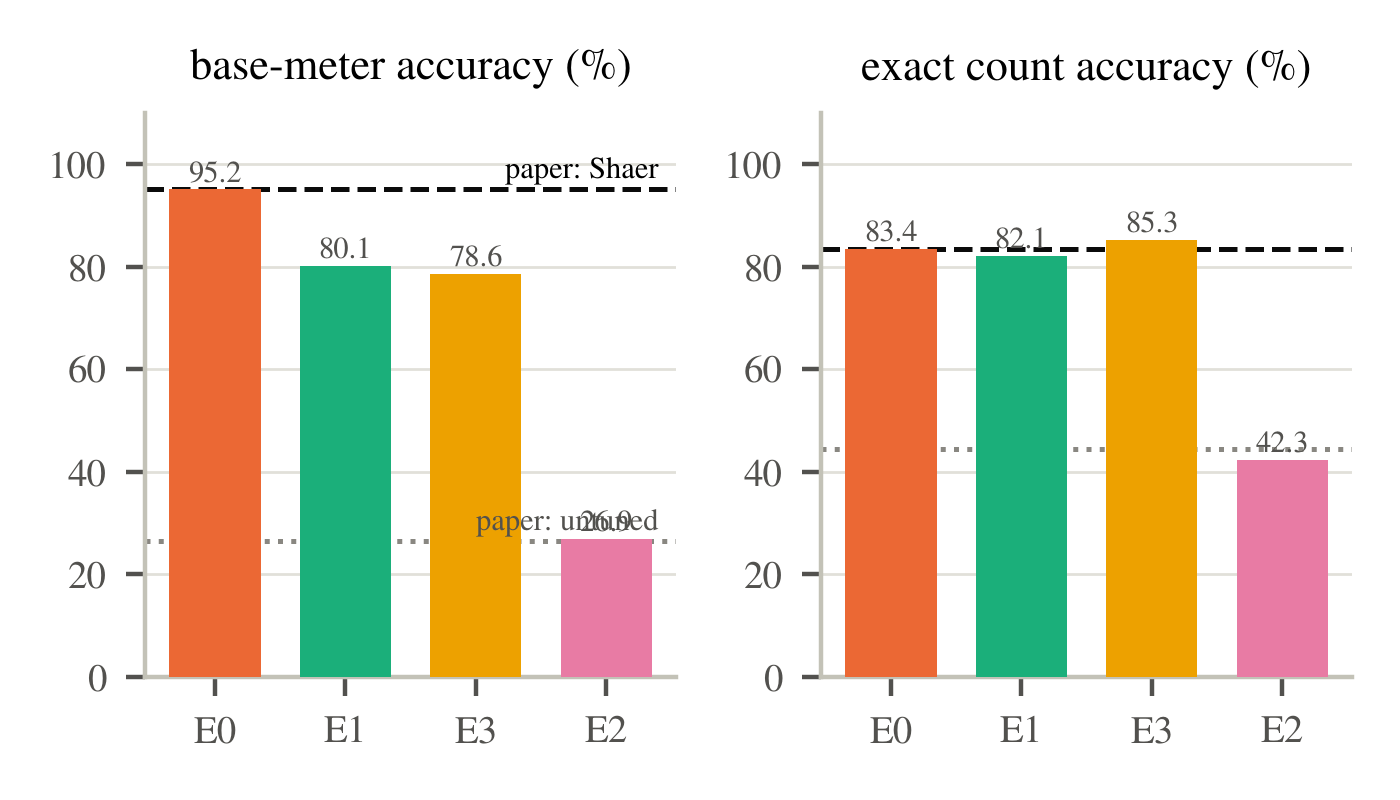
\includegraphics[width=\columnwidth]{fig_reproduction.png}
\caption{Base-meter accuracy and exact count accuracy of the four reproduction runs. Dashed lines: the paper's numbers
for Shaer and for the untuned model.}
\label{fig:repro}
\end{figure}

\textbf{E0 and E2 reproduce.} Re-scoring the released poems (E0) gives every published number exactly, so the
evaluation code and the BiLSTM behave as described. The untuned model (E2) lands within 0.4 points of the paper on
base-meter accuracy and within 2.2 points on exact count, which is within what one sampled generation can vary. One
detail is worth reporting: the paper's text describes base-meter accuracy as a majority vote over all bayts, but the
published 95.17\% is reproduced only by the prediction for the \emph{first} bayt. The majority vote gives 98.76\% on the
same poems.

\textbf{E1 and E3 do not reproduce the meter numbers.} New poems from the released adapter reach
\val{repEOneAcc}\% base-meter accuracy and a conformity of \val{repEOneConf}, about 15 points and 0.25 below the
released poems, while their length metrics match the paper closely. Our re-trained model (E3) behaves almost the same as
E1. Because E1 and E3 agree with each other and differ from E0 only on meter, the most likely cause is in the
generation pipeline rather than in the adapter weights. We see three candidate explanations, which we could not
separate within our compute budget. (i) \emph{Precision}: the adapter was trained on a 4-bit base model, while we
generated with the base model in bf16, so the adapter is applied to slightly different weights than it was trained
on. (ii) \emph{Engine and sampling}: the released poems may have been produced with a different inference engine such
as vLLM~\cite{kwon2023vllm} or with different sampling details; a 7B model sampled at temperature 0.55 is sensitive
to such differences. (iii) \emph{Checkpoint}: the released poems may come from a checkpoint other than the released
``best'' adapter. A further difference concerns training: our best evaluation loss (\val{ourBestLoss}) is higher than the
paper's (2.2074) and was reached earlier, at step \val{ourBestStep} (Fig.~\ref{fig:train}). Training ran across several
Colab sessions with resumption, which changes the data order and can change the optimiser state, and the paper does
not report the variance across seeds, so we cannot tell whether a gap of this size is unusual. We therefore treat
the released poems (E0) as the main sample, because they are what the paper's numbers describe, and use E1 and E3 as
additional samples.

\begin{figure}[t]
\centering
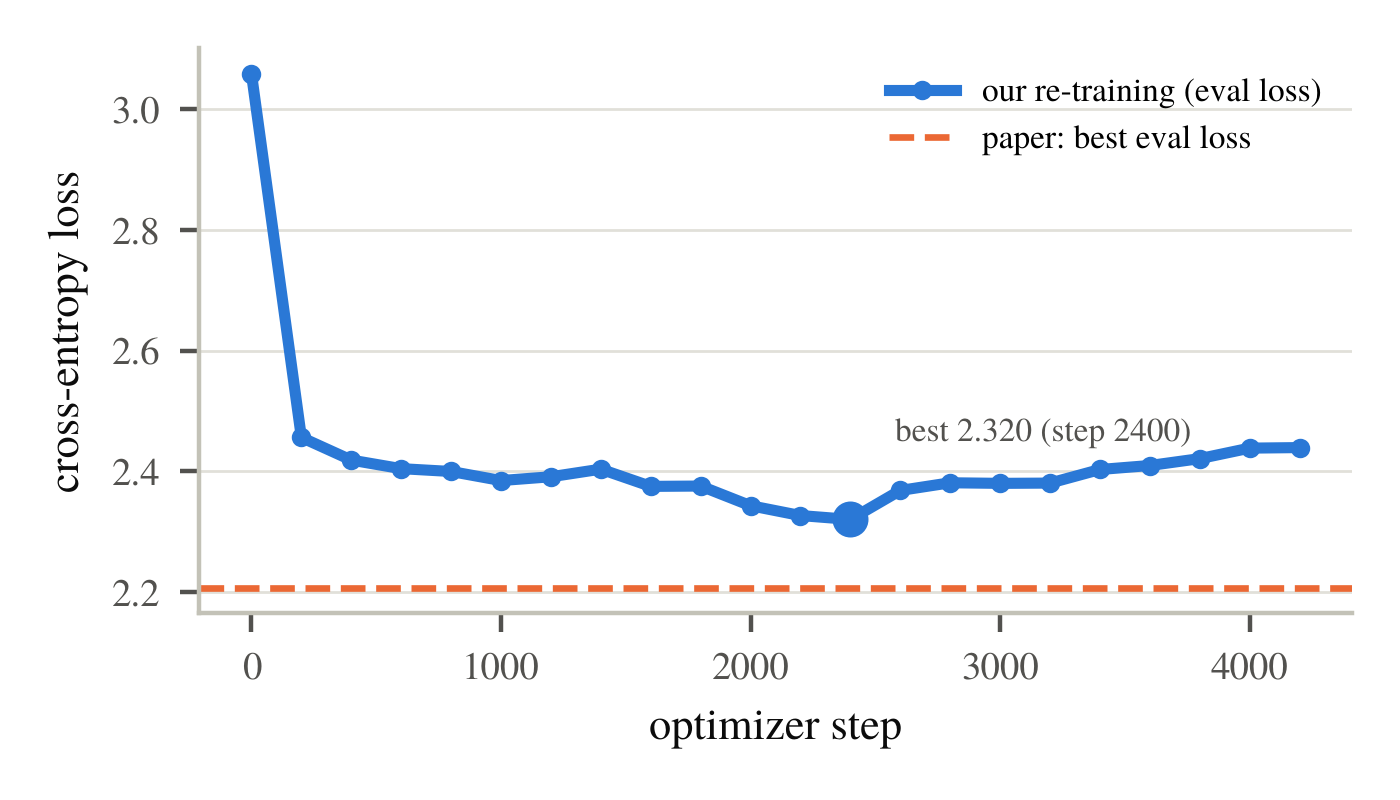
\includegraphics[width=\columnwidth]{fig_training_curve.png}
\caption{Evaluation loss of our re-training (E3) by optimiser step. The dashed line is the paper's best evaluation loss.}
\label{fig:train}
\end{figure}

\subsection{Measurement model: are the instruments valid and reliable?}
\label{sec:res-meas}
Before the strict numbers can be trusted, the verifier must accept real poems and reject broken ones. Section~\ref{sec:m1}
reported its validation: 87.1\% of human hemistichs accepted, 71.89\% of broken copies rejected, 100\% of planted rhyme
breaks flagged. The controls in Table~\ref{tab:m3} add a stronger check at poem level. When human poems are judged
against a wrong meter, \val{mCwmMeterOk}\% pass the meter check and \val{mCwmBaytOk}\% of bayts are accepted. When two
halves with different rhymes are joined, \val{mCmrRhymeOk}\% pass the rhyme check. The verifier can say ``no''.

Table~\ref{tab:agree} reports agreement between the instruments. Agreement between the BiLSTM and the verifier is low
for every system ($\kappa$ from \val{kEzeroVB} to \val{kRefVB}), because the BiLSTM accepts almost every bayt and nearly
all disagreement lies in one cell: bayts that the BiLSTM accepts and the verifier rejects. Agreement between the two
modes of the verifier is high ($\kappa = \val{kRefLB}$ on human poems), so the verdicts do not depend much on whether
written vowels are trusted.

\begin{table}[t]
\centering
\caption{Agreement between instruments, per bayt (Cohen's $\kappa$), and the share of BiLSTM-accepted bayts that the verifier rejects.}
\label{tab:agree}
\footnotesize
\begin{tabular}{@{}l r r r@{}}
\toprule
System & \shortstack{$\kappa$ BiLSTM\\vs.\ verifier} & \shortstack{$\kappa$ letters\\vs.\ binding} & \shortstack{BiLSTM yes,\\verifier no (\%)} \\
\midrule
Human & \textbf{\val{kRefVB}} & \textbf{\val{kRefLB}} & \textbf{\val{kRefBYesVNo}} \\
E0 released & \val{kEzeroVB} & \val{kEzeroLB} & \val{kEzeroBYesVNo} \\
E1 re-generated & \val{kEoneVB} & \val{kEoneLB} & \val{kEoneBYesVNo} \\
E3 re-trained & \val{kEthreeVB} & \val{kEthreeLB} & \val{kEthreeBYesVNo} \\
\bottomrule
\end{tabular}
\end{table}

\textbf{Reliability of the human ratings.} The quality construct of M6 is measured by four rating items and the five
judge items. Table~\ref{tab:reliab} is prepared for their reliability and validity; the values will be filled when the
human study is complete.

\begin{table}[t]
\centering
\caption{Reliability and discriminant validity of the quality measures (M6). Values pending the human study.}
\label{tab:reliab}
\footnotesize
\begin{tabular}{@{}>{\raggedright\arraybackslash}p{2.6cm} c c c c c@{}}
\toprule
Construct & Items & $\alpha_C$ & CR & AVE & Kripp.\ $\alpha$ \\
\midrule
Human rating (overall, meaning, fluency, meter) & 4 & \TBD & \TBD & \TBD & \TBD \\
LLM judge (5 items) & 5 & \TBD & \TBD & \TBD & -- \\
\midrule
\multicolumn{6}{@{}l}{HTMT (human rating, judge) = \TBD{} \quad threshold 0.85} \\
\bottomrule
\end{tabular}
\end{table}

\subsection{How valid are the poems? (H1, H2)}
Table~\ref{tab:m3} is the main result of the measurement study, and Fig.~\ref{fig:basever} shows its central contrast.

\begin{table*}[t]
\centering
\caption{Strict re-scoring of all systems (letters mode, margin 1.5). Rates in \% of 3,481 poems, except the first three
columns (\% of bayts). 95\% bootstrap intervals in brackets. Best model value per column in bold.}
\label{tab:m3}
\footnotesize
\setlength{\tabcolsep}{3.5pt}
\begin{tabular}{@{}l r r r r r r r r@{}}
\toprule
System & BiLSTM bayts & Verifier bayts & No reading & Meter valid & Rhyme valid & Exact length & Strictly valid & Strict (binding) \\
\midrule
Human & \val{mRefBilstmBaytOk} & \val{mRefBaytOk} & \val{mRefNoReading} & \val{mRefMeterOk} & \val{mRefRhymeOk} & \val{mRefCountExact} & \val{mRefStrictValid} \val{mRefStrictValidCI} & \val{mRefBindStrict} \\
\midrule
E0 released & \textbf{\val{mEzeroBilstmBaytOk}} & \val{mEzeroBaytOk} & \val{mEzeroNoReading} & \val{mEzeroMeterOk} & \val{mEzeroRhymeOk} & \val{mEzeroCountExact} & \val{mEzeroStrictValid} \val{mEzeroStrictValidCI} & \val{mEzeroBindStrict} \\
E1 re-generated & \val{mEoneBilstmBaytOk} & \val{mEoneBaytOk} & \val{mEoneNoReading} & \val{mEoneMeterOk} & \val{mEoneRhymeOk} & \val{mEoneCountExact} & \val{mEoneStrictValid} \val{mEoneStrictValidCI} & \val{mEoneBindStrict} \\
E3 re-trained & \val{mEthreeBilstmBaytOk} & \val{mEthreeBaytOk} & \val{mEthreeNoReading} & \val{mEthreeMeterOk} & \val{mEthreeRhymeOk} & \val{mEthreeCountExact} & \val{mEthreeStrictValid} \val{mEthreeStrictValidCI} & \val{mEthreeBindStrict} \\
E2 untuned & \val{mEtwoBilstmBaytOk} & \val{mEtwoBaytOk} & \val{mEtwoNoReading} & \val{mEtwoMeterOk} & \val{mEtwoRhymeOk} & \val{mEtwoCountExact} & \val{mEtwoStrictValid} \val{mEtwoStrictValidCI} & \val{mEtwoBindStrict} \\
\midrule
Control: wrong meter & -- & \val{mCwmBaytOk} & \val{mCwmNoReading} & \val{mCwmMeterOk} & \val{mCwmRhymeOk} & \val{mCwmCountExact} & \val{mCwmStrictValid} & -- \\
Control: mixed rhyme & -- & \val{mCmrBaytOk} & \val{mCmrNoReading} & \val{mCmrMeterOk} & \val{mCmrRhymeOk} & \val{mCmrCountExact} & \val{mCmrStrictValid} & -- \\
\bottomrule
\end{tabular}
\end{table*}

\begin{figure}[t]
\centering
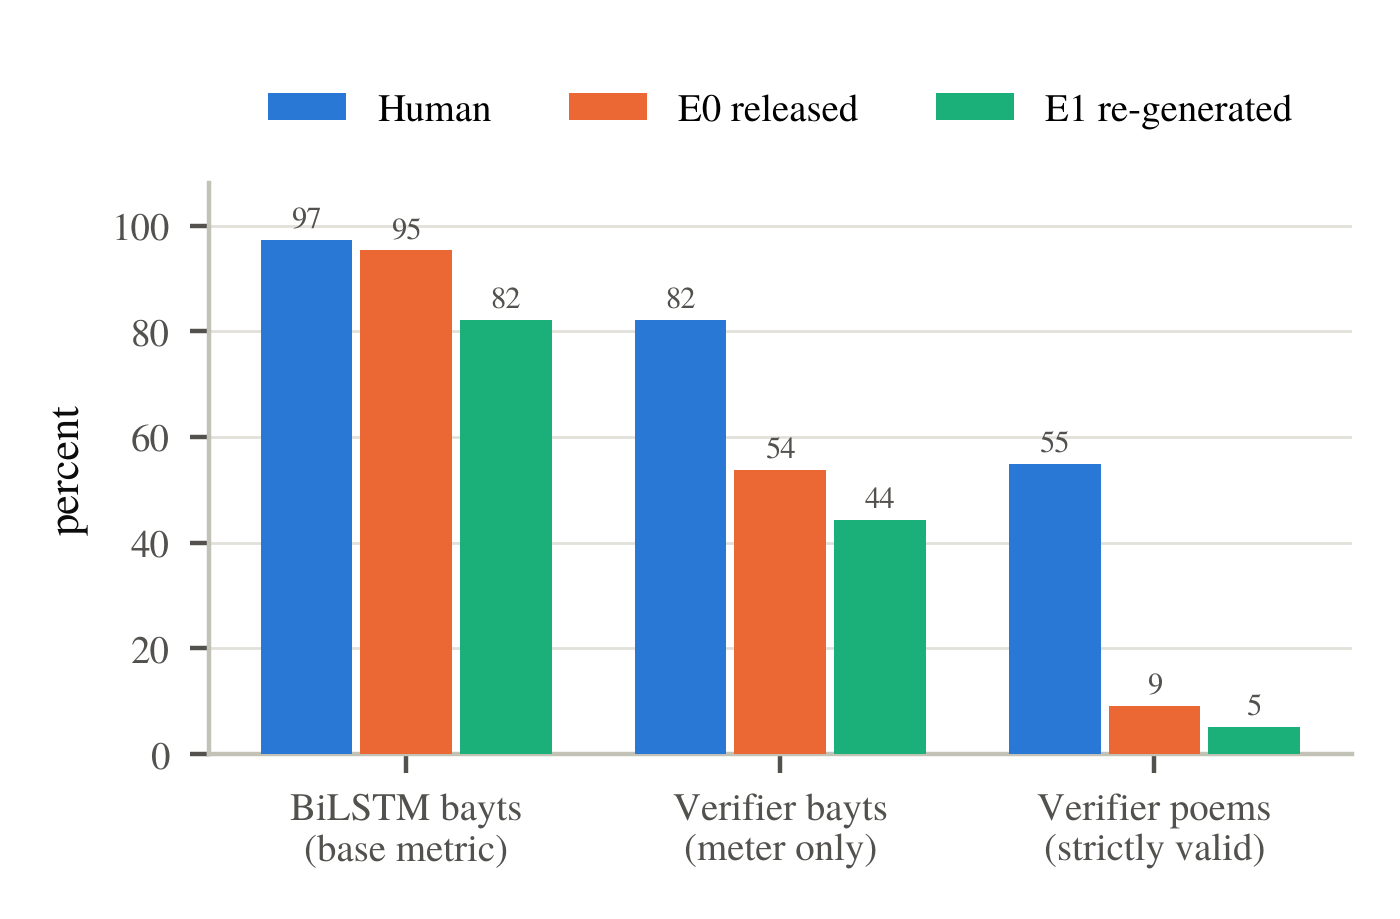
\includegraphics[width=\columnwidth]{fig_base_vs_verifier.png}
\caption{Bayts accepted by the BiLSTM, bayts accepted by the verifier, and strictly valid poems, per system. The BiLSTM
puts almost every system near the human level; the verifier does not.}
\label{fig:basever}
\end{figure}

\textbf{H1 is supported.} The BiLSTM accepts \val{mEzeroBilstmBaytOk}\% of the released Shaer bayts and the verifier
\val{mEzeroBaytOk}\%, a gap of 41.6 points. For human poems on the same prompts the gap is 15.2 points
(\val{mRefBilstmBaytOk}\% against \val{mRefBaytOk}\%). Part of the human gap is corpus noise and the verifier's own
errors (Section~\ref{sec:m1}), and it sets a reference for what the verifier rejects in correct poetry; the gap for
Shaer is almost three times larger. The margin-independent measure is clearer still: \val{mEzeroNoReading}\% of the
Shaer bayts have a hemistich with \emph{no reading at all} in the requested meter, against \val{mRefNoReading}\% of the
human bayts. Example 000013 in Table~\ref{tab:verifier-examples} is typical: a confident classifier decision on a line
that is a syllable away from the meter. The same pattern holds for our own runs E1 and E3 (Table~\ref{tab:m3}), so it is
not specific to the released poems. Of the poems that pass the base criterion \eqref{eq:base}, only
\val{gEzeroStrictGivenBase}\% are strictly valid.

\textbf{H2 is supported.} \val{mEzeroStrictValid}\% of the released poems are strictly valid, against
\val{mRefStrictValid}\% of the human poems; the paired difference is \val{mEzeroVsRefStrict}\pp{} (95\% CI), and
McNemar's test rejects equality ($\chi^2 = \val{mcEzeroChi}$, $p$ \val{mcEzeroP}). Every component contributes: the meter fails more often than in human poems,
the rhyme passes in only \val{mEzeroRhymeOk}\% of poems against \val{mRefRhymeOk}\%, and 16.6\% of poems have the wrong
length. Rhyme, which Shaer does not measure, is the largest single weakness. Binding mode, which also checks the
model's own vowel marks, lowers E0 to \val{mEzeroBindStrict}\%: the model often writes vowels that contradict the
meter.

\subsection{Length, meter and the structural model (H3)}
Fig.~\ref{fig:len} shows strict validity by requested length. The human poems lose validity with length too, because
every bayt is another chance for a corpus error or a false rejection, but the generated poems collapse much faster:
from \val{mEzeroLenA}\% for 1--3 bayts to \val{mEzeroLenB}\% for 4--6 and \val{mEzeroLenD}\% for 11--20 bayts.

\begin{figure}[t]
\centering
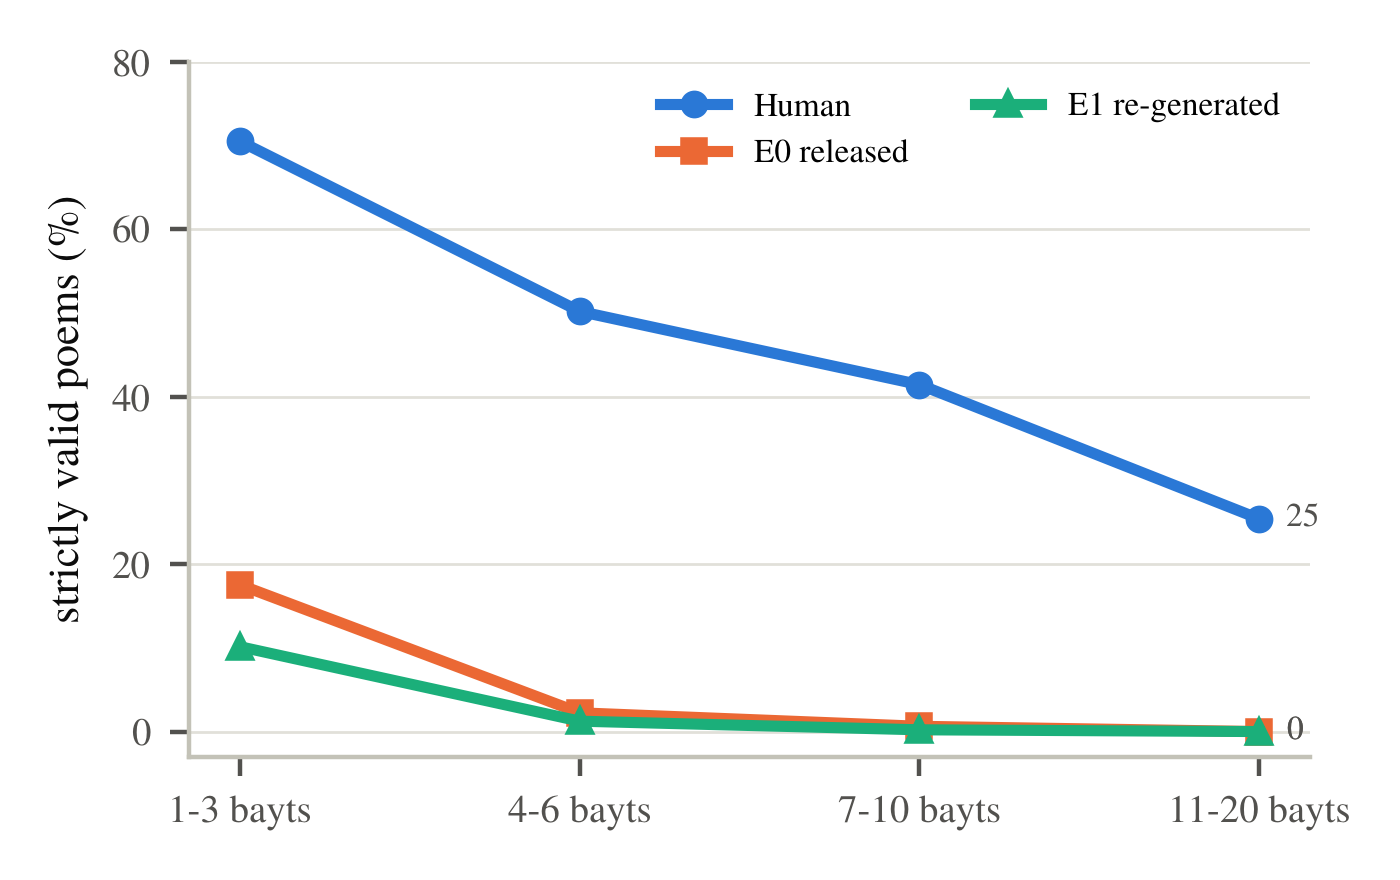
\includegraphics[width=\columnwidth]{fig_validity_by_length.png}
\caption{Strictly valid poems by requested length, with 95\% bootstrap intervals.}
\label{fig:len}
\end{figure}

Table~\ref{tab:logit} gives the structural model \eqref{eq:logit} for both criteria, fitted on the human poems and the
generated poems of E0, E1 and E3 together (E2 is left out because it almost never passes either criterion). Under both
criteria the human poems are far more likely to pass than E0, and every longer bucket is less likely to pass than
1--3 bayts, with odds ratios that shrink step by step. H3 is therefore supported, and the effect is large: under the
extended criterion, a poem of 11--20 bayts has about a tenth of the odds of a short one. Meter effects are smaller, but
two differences between the criteria are telling. Al-Khaf\={\i}f looks \emph{easier} than al-\d{T}aw\={\i}l under the
BiLSTM and harder under the verifier, and al-Mutaq\=arib is neutral under the BiLSTM but clearly harder under the
verifier. The choice of instrument changes not only the level of validity but also which meters look difficult.

\begin{table*}[t]
\centering
\caption{Structural model: logistic regression of validity on system, requested length and meter, for the base
criterion (BiLSTM, exact length) and the extended criterion (strict validity). Reference levels: E0, 1--3 bayts,
al-\d{T}aw\={\i}l. $\beta$ in bold when the 95\% cluster-bootstrap interval (5,000 resamples) excludes 0.}
\label{tab:logit}
\footnotesize
\begin{tabular}{@{}l r c r r c r@{}}
\toprule
& \multicolumn{3}{c}{Base criterion $G(p)$} & \multicolumn{3}{c}{Extended criterion $V(p)$} \\
\cmidrule(lr){2-4}\cmidrule(lr){5-7}
Term & $\beta$ & 95\% CI & OR & $\beta$ & 95\% CI & OR \\
\midrule
\rowsinput{generated/tab_logit.tex}
\bottomrule
\end{tabular}
\end{table*}

\subsection{Summary of hypotheses}
Table~\ref{tab:hyp} summarises the hypotheses and the reproduction claims. Three measurement hypotheses are supported.
The five improvement hypotheses are pending their runs; their pre-registered predictions are fixed in the project
repository and their results will be read against them.

\begin{table}[t]
\centering
\caption{Hypotheses and reproduction claims: results.}
\label{tab:hyp}
\footnotesize
\begin{tabularx}{\columnwidth}{@{}l >{\raggedright\arraybackslash}X >{\raggedright\arraybackslash}p{1.25cm}@{}}
\toprule
& Evidence & Result \\
\midrule
R1 & E0 equals all four published metrics & Reproduced \\
R2 & E2 within 0.4 / 2.2 points of the paper & Reproduced \\
R3 & E1 base-meter accuracy \val{repEOneAcc}\% vs.\ 95.17\% & Not reproduced \\
R4 & E3 loss \val{ourBestLoss} vs.\ 2.2074; length metrics match & Partly \\
\midrule
H1 & Verifier--BiLSTM gap 41.6 vs.\ 15.2 points; no reading \val{mEzeroNoReading}\% vs.\ \val{mRefNoReading}\% & Supported \\
H2 & $\Delta = \val{mEzeroVsRefStrict}$\pp, McNemar $p$ \val{mcEzeroP} & Supported \\
H3 & All length coefficients $<0$, CIs exclude 0 & Supported \\
H4 & Search vs.\ matched best-of-$N$: \TBD & \pending{pending M4} \\
H5 & Gain under BiLSTM and binding mode: \TBD & \pending{pending M4} \\
H6 & 2a vs.\ E3, rhyme pass: \TBD & \pending{pending M5} \\
H7 & 2c vs.\ 2a, strict validity: \TBD & \pending{pending M5} \\
H8 & Judge, distinct-2, copying within bounds: \TBD & \pending{pending M6} \\
\bottomrule
\end{tabularx}
\end{table}

\subsection{Improvement results (pending)}
\label{sec:res-pending}
The M4--M6 runs need many GPU hours and paid judge calls and were in progress when this version was written.
Table~\ref{tab:pending} is the table that will receive their results, and Fig.~\ref{fig:m4pred} shows the
predictions for M4 that were registered before any run.

\begin{table}[t]
\centering
\caption{Results of the improvement studies on the test prompts (placeholders until the runs finish).}
\label{tab:pending}
\footnotesize
\setlength{\tabcolsep}{3pt}
\begin{tabular}{@{}l r r r r r@{}}
\toprule
System & Budget & Strict & BiLSTM bayts & Rhyme & Judge mean \\
\midrule
E3 (one sample) & 1.0$\times$ & \val{mEthreeStrictValid} & \val{mEthreeBilstmBaytOk} & \val{mEthreeRhymeOk} & \TBD \\
M4 best-of-$N$ (matched) & \TBD & \TBD & \TBD & \TBD & \TBD \\
M4 hemistich search & \TBD & \TBD & \TBD & \TBD & \TBD \\
M5 2a (raw\={\i} in prompt) & 1.0$\times$ & \TBD & \TBD & \TBD & \TBD \\
M5 2b (clean data) & 1.0$\times$ & \TBD & \TBD & \TBD & \TBD \\
M5 2c (one round) & 1.0$\times$ & \TBD & \TBD & \TBD & \TBD \\
Human & -- & \val{mRefStrictValid} & \val{mRefBilstmBaytOk} & \val{mRefRhymeOk} & \TBD \\
\bottomrule
\end{tabular}
\end{table}

\begin{figure}[t]
\centering
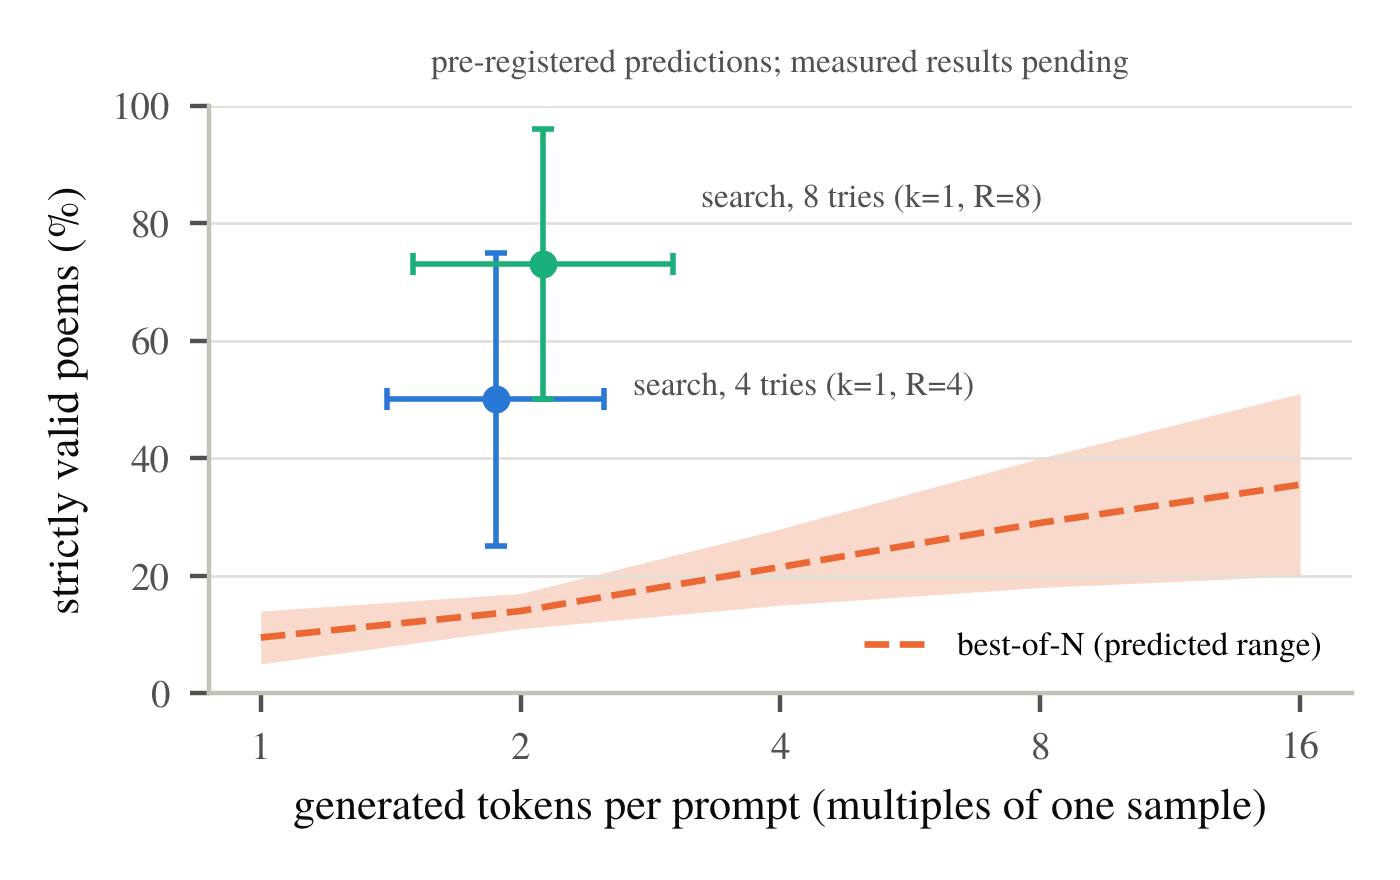
\includegraphics[width=\columnwidth]{fig_m4_predictions.png}
\caption{Pre-registered predictions for M4: strict validity of best-of-$N$ (band) and of the hemistich search (bars
show the predicted ranges of validity and budget). Measured values will be added when the runs finish.}
\label{fig:m4pred}
\end{figure}

\subsection{Discussion}
The results answer RQ1 and RQ2 clearly. Shaer's published numbers are a faithful description of its released poems,
but a new generation with the released adapter, and a re-training with the released recipe, both land well below them
on meter; reproducing an LLM generation result needs more than the weights and the script, and papers should state the
precision, engine and checkpoint used for generation. More importantly, the published meter metric measures something
weaker than metrical correctness. The BiLSTM answers ``which meter is this closest to?'', and for generated text that
question has a confident answer even when the line is broken. Once every hemistich is scanned and rhyme and length are
checked together, fewer than one released poem in ten is fully correct, and long poems are almost never correct. The
problem is not specific to Shaer: any system evaluated or rewarded by a closed-set classifier inherits the same blind
spot, including the reinforcement-learning adapters that Shaer releases. A verifier that can reject, explain and
localise errors is the missing instrument, and it also opens the door to the improvements of RQ3, because the same
check can guide decoding and select training data.

\section{Robustness Checks}
\label{sec:robust}

\subsection{Nested model comparison}
Table~\ref{tab:nested} compares three nested versions of the structural model \eqref{eq:logit} for each criterion:
S1 with the system only, S2 adding the requested length and S3 adding the meter. Fig.~\ref{fig:nested} plots their fit.
Length adds by far the most to both models, and the meter adds a smaller but significant amount; S3 has the lowest AIC
under both criteria. The system effect alone explains about twice as much under the extended criterion as under the
base criterion, which is H1 seen from another angle: the base criterion hides most of the difference between the human
and generated poems.

\begin{table}[t]
\centering
\caption{Nested structural models (likelihood-ratio tests against the previous step). Lowest AIC per criterion in bold.}
\label{tab:nested}
\scriptsize
\setlength{\tabcolsep}{2.5pt}
\begin{tabular}{@{}l l r r r r r@{}}
\toprule
Criterion & Model & $k$ & $R^2_{\mathrm{McF}}$ & AIC & LR ($df$) & $p$ \\
\midrule
\rowsinput{generated/tab_nested.tex}
\bottomrule
\end{tabular}
\end{table}

\begin{figure}[t]
\centering
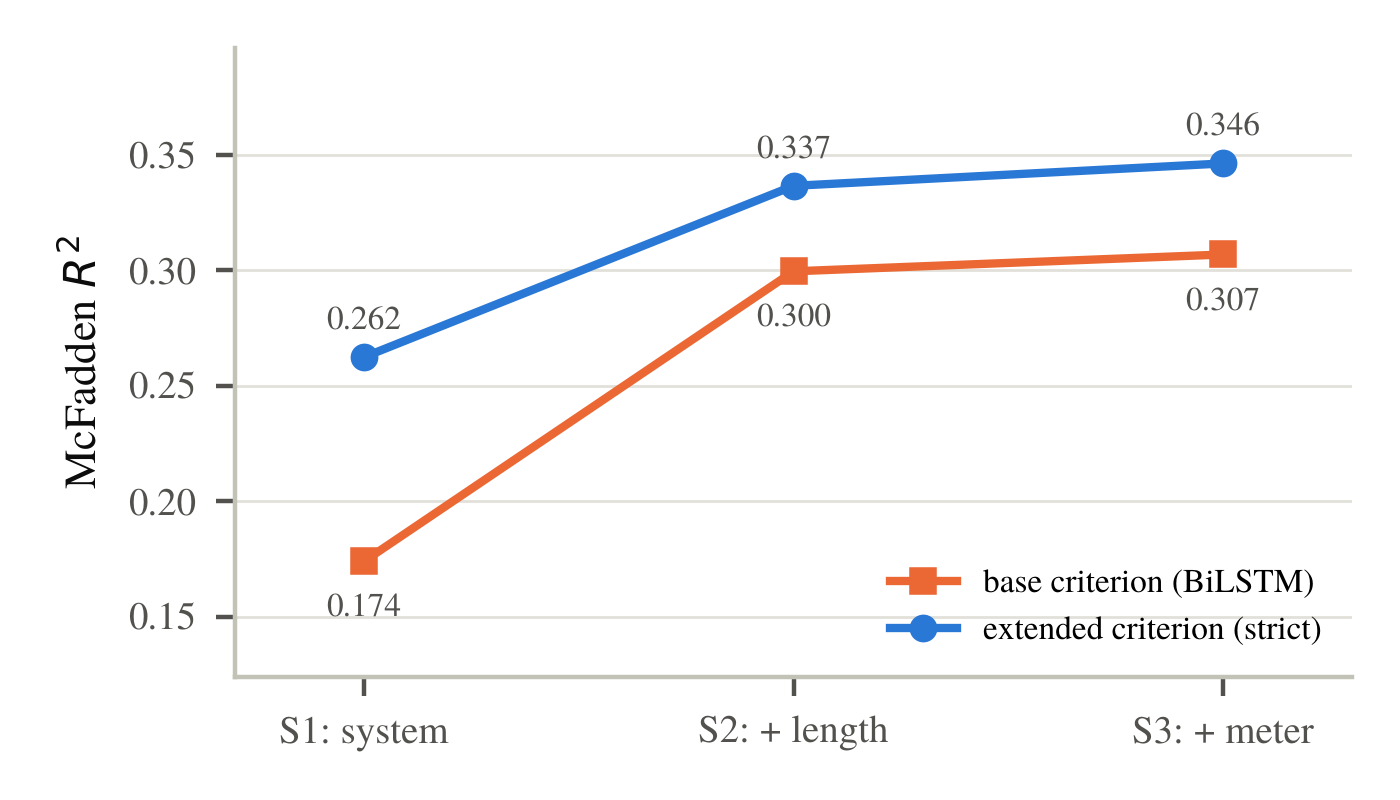
\includegraphics[width=\columnwidth]{fig_nested.png}
\caption{Fit of the nested structural models (McFadden $R^2$) for the base and the extended criterion.}
\label{fig:nested}
\end{figure}

\subsection{Alternative specifications of validity}
The extended criterion has several parts and one tuned setting, the margin $\delta$. Table~\ref{tab:variants} and
Fig.~\ref{fig:robust} recompute strict validity with one part removed or changed at a time. The gap between the human
poems and E0 survives every variant. Removing the rhyme check raises E0 the most (to \val{vEzeroNoRhyme}\%), which
confirms that rhyme is its largest weakness. Removing the length check changes little, because most length errors come
together with meter or rhyme errors. Accepting any form of the requested meter changes almost nothing. The margin
matters for human poems, whose rejections are mostly of the margin kind (Section~\ref{sec:m1}), and much less for E0,
whose failures are mostly hemistichs with no reading in the meter: without any margin, E0 rises only to
\val{vEzeroNoMargin}\% while the human poems rise to \val{vRefNoMargin}\%. So the low validity of the generated poems is
not an artefact of the margin. Binding mode is stricter for both. Finally, the base criterion passes
\val{vEzeroBaseBilstm}\% of E0 poems, eight times the strict rate.

\begin{table}[t]
\centering
\caption{Strict validity (\%) under alternative specifications. Each row changes one part of the extended criterion.}
\label{tab:variants}
\footnotesize
\setlength{\tabcolsep}{3pt}
\begin{tabular}{@{}l r r r r r r@{}}
\toprule
Specification & Human & E0 & E1 & E3 & C-wm & C-mr \\
\midrule
Full (margin 1.5) & \val{vRefFull} & \val{vEzeroFull} & \val{vEoneFull} & \val{vEthreeFull} & \val{vCwmFull} & \val{vCmrFull} \\
-- rhyme check & \val{vRefNoRhyme} & \val{vEzeroNoRhyme} & \val{vEoneNoRhyme} & \val{vEthreeNoRhyme} & \val{vCwmNoRhyme} & \val{vCmrNoRhyme} \\
-- length check & \val{vRefNoLength} & \val{vEzeroNoLength} & \val{vEoneNoLength} & \val{vEthreeNoLength} & \val{vCwmNoLength} & \val{vCmrNoLength} \\
any form of the meter & \val{vRefAnyForm} & \val{vEzeroAnyForm} & \val{vEoneAnyForm} & \val{vEthreeAnyForm} & \val{vCwmAnyForm} & \val{vCmrAnyForm} \\
margin 1.0 & \val{vRefMarginOne} & \val{vEzeroMarginOne} & \val{vEoneMarginOne} & \val{vEthreeMarginOne} & \val{vCwmMarginOne} & \val{vCmrMarginOne} \\
margin 3.0 & \val{vRefMarginThree} & \val{vEzeroMarginThree} & \val{vEoneMarginThree} & \val{vEthreeMarginThree} & \val{vCwmMarginThree} & \val{vCmrMarginThree} \\
no margin & \val{vRefNoMargin} & \val{vEzeroNoMargin} & \val{vEoneNoMargin} & \val{vEthreeNoMargin} & \val{vCwmNoMargin} & \val{vCmrNoMargin} \\
binding mode & \val{vRefBinding} & \val{vEzeroBinding} & \val{vEoneBinding} & \val{vEthreeBinding} & -- & -- \\
\midrule
base criterion (BiLSTM) & \val{vRefBaseBilstm} & \val{vEzeroBaseBilstm} & \val{vEoneBaseBilstm} & \val{vEthreeBaseBilstm} & -- & -- \\
\bottomrule
\end{tabular}
\end{table}

\begin{figure*}[t]
\centering
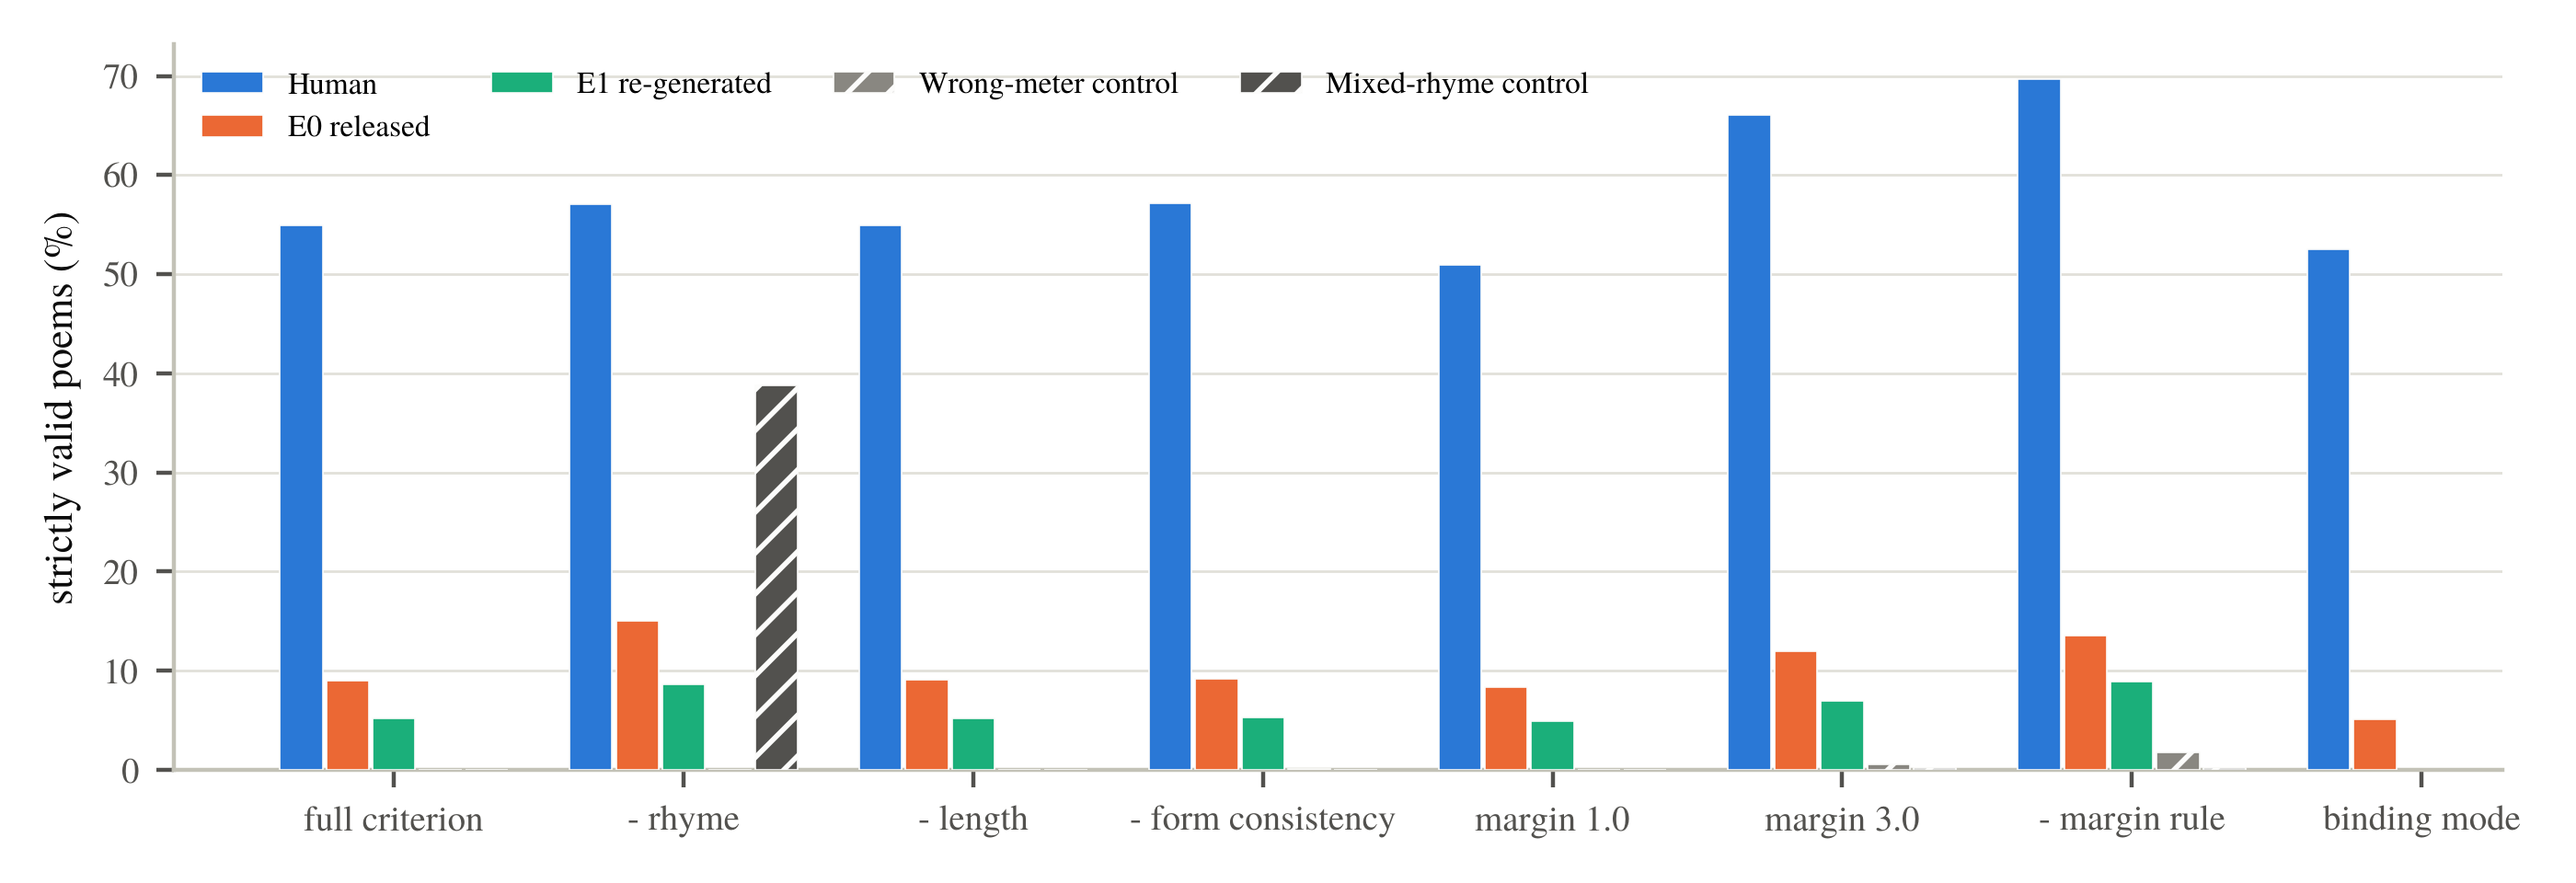
\includegraphics[width=0.8\textwidth]{fig_robustness.png}
\caption{Strict validity under the alternative specifications of Table~\ref{tab:variants}. Hatched bars are the control
samples, which stay near zero under every specification that keeps the part they break.}
\label{fig:robust}
\end{figure*}

\subsection{Subsample checks}
\textbf{Independent generations.} The findings on the released poems were repeated on our own poems, E1 (released
adapter) and E3 (re-trained). Both have a large gap between the BiLSTM and the verifier, a strict-validity rate far
below the human poems, and the same decline with length (Tables~\ref{tab:m3} and~\ref{tab:variants}).
\textbf{Short poems.} Restricted to the 1,668 prompts of 1--3 bayts, where length errors are rare, E0 is still strictly
valid for only \val{mEzeroLenA}\% against \val{mRefLenA}\% of human poems, so the gap is not produced by long poems
alone.

\subsection{Common method bias and multiple testing}
In survey research, common method bias arises when the same instrument measures both sides of a
relation~\cite{podsakoff2003cmb}. The analogue here is that the verifier both selects poems (M4, M5) and scores them.
We address it in three ways: (i) the measurement results (H1--H3) involve no selection at all; (ii) every improvement
is also scored by instruments that did not select the poems, namely the BiLSTM, the binding mode and the LLM judge
(H5); and (iii) the human study is blinded. For multiple testing, the hypotheses are grouped into families (measurement,
M4, M5, M6) and Holm's correction~\cite{holm1979simple} is applied within each family. The measurement results have
$p<0.001$ and are unaffected by the correction.

\section{Practical Implications and Case Study}
\label{sec:case}

\subsection{Practical implications}
Three implications follow for anyone who builds or buys an Arabic poetry generator. First, \emph{a classifier score is
not a quality gate}: a system that reports 95\% meter accuracy may deliver fewer than 10\% fully correct poems. Second,
\emph{validity must be measured per poem and jointly}: meter, rhyme and length fail together and compound with length,
so per-metric averages hide most failures. Third, \emph{a rule-based verifier is cheap to run and explains its
verdicts}: it needs no GPU, it names the broken foot, and it can be placed in front of human editors so that their time
goes to meaning rather than to scansion.

\subsection{Case study: a textbook publisher}
To make these points concrete we walk through an \emph{illustrative} scenario. The organisation is a composite, not a
real company, and the numbers are taken from our measurements.

\textbf{Setting.} An educational publisher prepares a secondary-school Arabic literature textbook. The prosody chapter
needs 200 short original poems (two or three bayts each) in six common meters, on topics from the curriculum, for
students to scan as exercises. A poem with a broken hemistich is worse than no poem: students would learn a wrong
pattern, and teachers would lose trust in the book. The publisher has two editors who know prosody and a small budget
of cloud GPU time.

\textbf{Option A: the generator and its published metric.} The team generates one poem per request and keeps the poems
that pass the base criterion. By our measurements, \val{vEzeroBaseBilstm}\% of the released poems pass it, so
the team quickly has 200 ``validated'' poems. But only \val{gEzeroStrictGivenBase}\% of poems that pass this criterion are
strictly valid. The editors must therefore scan every poem by hand and will reject most of them, often for a rhyme
fault that no metric flagged. The saving from automation disappears.

\textbf{Option B: a verifier gate with resampling.} The team puts the verifier between the generator and the editors
(Fig.~\ref{fig:case}). A poem reaches an editor only if it is strictly valid; otherwise the request is sampled again,
up to a budget. For 1--3-bayt poems the released model is strictly valid \val{mEzeroLenA}\% of the time, so a valid poem
needs about six samples on average if samples are independent (an optimistic assumption, since some prompts are harder
than others). At the 2.4\,s per poem we measured for generation on an L4 GPU, 200 valid poems cost roughly
$200 \times 6 \times 2.4\,\mathrm{s} \approx 48$ minutes of GPU time. The editors now review only meaning, tone and
suitability for students. When a request exhausts its budget, the verifier's report (the hemistich, the nearest valid
pattern and the broken foot) lets an editor repair the line by hand in minutes.

\textbf{Option C: hemistich search (pending).} With the M4 search, the generator repairs each hemistich as it writes,
so the predicted cost per valid poem is lower than in Option B, and poems of four or more bayts, for which Option B
would need about 45 samples each, become feasible. The measured cost is \pending{pending M4}.

\begin{figure}[t]
\centering
\begin{tikzpicture}[
  font=\scriptsize,
  st/.style={draw=black!70, rounded corners=2pt, fill=#1, align=center, text width=1.75cm, minimum height=0.95cm, inner sep=2pt},
  st/.default={blue!6},
  dec/.style={draw=black!70, diamond, aspect=1.6, fill=yellow!12, align=center, inner sep=0.5pt, font=\scriptsize},
  arr/.style={-{Stealth[length=2mm]}, thick, draw=black!70}]
\node[st={gray!10}] (req) {Request: meter, length, topic, raw\={\i}};
\node[st, right=0.35cm of req] (gen) {Generator (Shaer adapter)};
\node[dec, right=0.35cm of gen] (ver) {Verifier\\ valid?};
\node[st={green!8}, right=0.35cm of ver] (ed) {Editor: meaning, tone};
\node[st={green!8}, below=0.6cm of ed] (book) {Textbook};
\node[dec, below=0.7cm of gen] (bud) {Budget\\ left?};
\node[st={orange!10}, left=0.35cm of bud] (fix) {Editor repairs from report};
\draw[arr] (req) -- (gen);
\draw[arr] (gen) -- (ver);
\draw[arr] (ver) -- node[above, font=\scriptsize] {yes} (ed);
\draw[arr] (ed) -- (book);
\draw[arr] (ver) |- node[pos=0.25, right, font=\scriptsize] {no} (bud);
\draw[arr] (bud) -- node[right, font=\scriptsize] {yes} (gen);
\draw[arr] (bud) -- node[above, font=\scriptsize] {no} (fix);
\draw[arr] (fix.south) |- ($(book.south west)+(0,0.2)$);
\end{tikzpicture}
\caption{Case-study scenario: the verifier as a quality gate between the generator and the human editors.}
\label{fig:case}
\end{figure}

\textbf{Lessons.} The publisher's decision depends on the metric it trusts. Under the published metric the generator
looks ready for use; under the strict criterion it is a useful drafting tool that needs a verifier in the loop. The
gate also changes the editors' work from scanning lines to judging content, which is where human judgement is most
valuable.

\section{Ethics, Limitations and Threats to Validity}
\label{sec:ethics}

\subsection{Ethical considerations}
\textbf{Data.} The study uses the public Ashaar corpus as released by the Shaer authors and the models released by
their authors under their licences; the base model Yehia-7B was used with the permission of its authors. The corpus
consists of classical poems and contains no personal data. Generated poems are always labelled as machine-generated in
our outputs and are not presented as the work of any poet.

\textbf{Human participants.} The measurement results in this paper involve no human participants. The planned human
study of M6 will involve adult volunteers who read and rate poems. It will follow three principles. \emph{Informed
consent}: every rater will read and sign the consent form in Appendix~\ref{app:consent} before taking part.
\emph{Voluntary participation}: raters may stop at any time without giving a reason, and their partial ratings will be
deleted on request. \emph{Anonymity}: ratings will be stored under a random rater code, no names or contact details
will be stored with them, and only aggregate results will be published. The study will be submitted to the
\pending{institutional ethics committee} before any data are collected.

\textbf{Cultural care.} Classical Arabic poetry is a living cultural heritage. A tool that writes it at scale can
devalue the work of poets if it is presented as a replacement. We present the generator as a drafting aid and the
verifier as a teaching and checking tool.

\subsection{Limitations and threats to validity}
\textbf{Construct validity.} Strict validity depends on the verifier. Its rules were checked against textbooks and
two open implementations, but not yet signed off by a prosodist (M2). On human poems it rejects some correct lines,
mostly because of the margin rule on undiacritised text, so the human rates are lower bounds. We reduce this threat by
reporting the margin-independent no-reading rate, varying the margin, using binding mode and using controls.

\textbf{Internal validity.} The E1 and E3 gaps to the paper have several possible causes that we could not separate.
The verifier was developed while looking at the released poems, which could bias it against them; the margin and the
lexicon were therefore fixed on the evaluation and training splits only, and the controls show that it rejects broken
human poems as well.

\textbf{External validity.} The results cover one model family (Yehia-7B with QLoRA), one corpus and 13 of the 16
meters. Generators with other tokenisers or larger models may behave differently, and rare meters have few test
prompts.

\textbf{Statistical conclusion validity.} All main comparisons are paired, use 3,481 prompts with 5,000-resample
bootstrap intervals and have high power (Section~\ref{sec:power}). Each system was sampled once per prompt, so variation
between generation runs is not captured by the intervals; E1 and E3 give a partial view of it.

\textbf{Pending results.} H4--H8 are untested in this version. Their predictions were fixed before the runs so that the
results cannot be fitted to them afterwards.

\section{Conclusion}
\label{sec:conclusion}
We reproduced Shaer, a fine-tuned LLM for controlled classical Arabic poetry, and examined what its meter metric
measures. Re-scoring the released poems reproduced every published number, and the untuned baseline reproduced
closely, but new generations from the released adapter and a full re-training scored about 15 points lower on
base-meter accuracy, which points to undocumented details of the generation pipeline. We then built a formal verifier
of Arabic prosody and showed that the published metric overstates validity: \val{mEzeroStrictValid}\% of the released
poems are strictly valid in meter, rhyme and length, against \val{mRefStrictValid}\% of the human poems for the same
prompts, \val{mEzeroNoReading}\% of the bayts that the classifier accepts contain a hemistich that cannot be read in the
requested meter at all, and validity collapses as poems get longer. These findings held across nested models,
alternative specifications, independent generation runs and control samples.

Two lessons reach beyond this system. Generators of formal verse should be evaluated, and rewarded, by instruments that
can reject, not only classify. And reproductions of LLM generation results need the generation precision, engine and
checkpoint, not only the weights and the training script. The verifier, the analysis code and all predictions are
public. Future work will complete the pre-registered extensions (hemistich search, self-training and the quality study),
obtain an expert-labelled gold set for the verifier, and carry the approach to Urdu and Persian verse, whose meters
derive from the same tradition.


\bibliographystyle{IEEEtran}
\bibliography{references}

\appendices
\section{Consent Form for the Human Rating Study}
\label{app:consent}

\noindent\textbf{Study title:} Quality of machine-generated classical Arabic poetry.\\
\textbf{Researcher:} Muhammad Shahbaz, \pending{department and university}; contact \pending{email}.\\
\textbf{Supervisor:} \pending{name}.

\smallskip
\noindent\textbf{What the study is about.} We are studying computer programs that write classical Arabic poems. You
will read about 120 short poems. Some were written by people and some by computer programs; you will not be told which.

\smallskip
\noindent\textbf{What you will do.} For each poem you will give four ratings from 1 (very poor) to 5 (excellent):
overall quality, meaning, fluency, and how the meter sounds when read aloud. This takes about two hours and can be done
in several sittings.

\smallskip
\noindent\textbf{Voluntary participation.} Taking part is voluntary. You may stop at any time without giving a reason
and without any consequence. If you stop, you may ask us to delete the ratings you have given.

\smallskip
\noindent\textbf{Anonymity and data.} Your ratings will be stored under a random code. Your name and contact details
will be kept separately and will not be linked to your ratings in any file we share or publish. Only averages over
raters will be published. The data will be kept for \pending{period} and then deleted.

\smallskip
\noindent\textbf{Risks and benefits.} There are no known risks beyond the time spent. Some poems may contain classical
themes such as war or loss. There is no direct benefit to you; the results will help to build better tools for Arabic
literature and teaching.

\smallskip
\noindent\textbf{Questions.} You can contact the researcher or \pending{the ethics committee} at any time.

\smallskip
\noindent\textbf{Consent.} I have read this information, I have had the chance to ask questions, and I agree to take
part.

\smallskip
\noindent Rater code: \rule{2.5cm}{0.4pt} \quad Signature: \rule{3cm}{0.4pt} \quad Date: \rule{2cm}{0.4pt}

\section{Reproducibility Checklist}
\label{app:repro}
Following Pineau et al.~\cite{pineau2021reproducibility}, we list what is needed to repeat every number in this paper.
\begin{itemize}
\item \textbf{Code:} the baseline notebook \texttt{colab/reproduce\_shaer\_a100.ipynb} (E0--E3) and the research notebook
\texttt{prosody-verifier/prosody\_main.ipynb} (M0--M6), both runnable on Google Colab; the verifier in
\texttt{prosody-verifier/prosody/}; the analysis in \texttt{prosody-verifier/paper/scripts/analysis.py}.
\item \textbf{Data:} the Shaer splits and released poems from the authors' Hugging Face repositories; the pronunciation
lexicon built from the training split and shipped with the code.
\item \textbf{Versions:} every verifier record carries the hashes of the verifier and the lexicon; the notebooks check
their own version against the code.
\item \textbf{Randomness:} generation seed 42; bootstrap seed 7; M4 development subset seed 2026.
\item \textbf{Pre-registration:} the expectations of M3--M6 were committed to the repository before the corresponding
runs, in \texttt{prosody-verifier/validation/}.
\item \textbf{Tests:} the repository's test suite covers the rule tables (textbook equalities), the reading rules, the
rhyme rules, the search, the data builders and the report generators.
\end{itemize}


\end{document}
